\documentclass[1p]{elsarticle_modified}
%\bibliographystyle{elsarticle-num}

%\usepackage[colorlinks]{hyperref}
%\usepackage{abbrmath_seonhwa} %\Abb, \Ascr, \Acal ,\Abf, \Afrak
\usepackage{amsfonts}
\usepackage{amssymb}
\usepackage{amsmath}
\usepackage{amsthm}
\usepackage{scalefnt}
\usepackage{amsbsy}
\usepackage{kotex}
\usepackage{caption}
\usepackage{subfig}
\usepackage{color}
\usepackage{graphicx}
\usepackage{xcolor} %% white, black, red, green, blue, cyan, magenta, yellow
\usepackage{float}
\usepackage{setspace}
\usepackage{hyperref}

\usepackage{tikz}
\usetikzlibrary{arrows}

\usepackage{multirow}
\usepackage{array} % fixed length table
\usepackage{hhline}

%%%%%%%%%%%%%%%%%%%%%
\makeatletter
\renewcommand*\env@matrix[1][\arraystretch]{%
	\edef\arraystretch{#1}%
	\hskip -\arraycolsep
	\let\@ifnextchar\new@ifnextchar
	\array{*\c@MaxMatrixCols c}}
\makeatother %https://tex.stackexchange.com/questions/14071/how-can-i-increase-the-line-spacing-in-a-matrix
%%%%%%%%%%%%%%%

\usepackage[normalem]{ulem}

\newcommand{\msout}[1]{\ifmmode\text{\sout{\ensuremath{#1}}}\else\sout{#1}\fi}
%SOURCE: \msout is \stkout macro in https://tex.stackexchange.com/questions/20609/strikeout-in-math-mode

\newcommand{\cancel}[1]{
	\ifmmode
	{\color{red}\msout{#1}}
	\else
	{\color{red}\sout{#1}}
	\fi
}

\newcommand{\add}[1]{
	{\color{blue}\uwave{#1}}
}

\newcommand{\replace}[2]{
	\ifmmode
	{\color{red}\msout{#1}}{\color{blue}\uwave{#2}}
	\else
	{\color{red}\sout{#1}}{\color{blue}\uwave{#2}}
	\fi
}

\newcommand{\Sol}{\mathcal{S}} %segment
\newcommand{\D}{D} %diagram
\newcommand{\A}{\mathcal{A}} %arc


%%%%%%%%%%%%%%%%%%%%%%%%%%%%%5 test

\def\sl{\operatorname{\textup{SL}}(2,\Cbb)}
\def\psl{\operatorname{\textup{PSL}}(2,\Cbb)}
\def\quan{\mkern 1mu \triangleright \mkern 1mu}

\theoremstyle{definition}
\newtheorem{thm}{Theorem}[section]
\newtheorem{prop}[thm]{Proposition}
\newtheorem{lem}[thm]{Lemma}
\newtheorem{ques}[thm]{Question}
\newtheorem{cor}[thm]{Corollary}
\newtheorem{defn}[thm]{Definition}
\newtheorem{exam}[thm]{Example}
\newtheorem{rmk}[thm]{Remark}
\newtheorem{alg}[thm]{Algorithm}

\newcommand{\I}{\sqrt{-1}}
\begin{document}

%\begin{frontmatter}
%
%\title{Boundary parabolic representations of knots up to 8 crossings}
%
%%% Group authors per affiliation:
%\author{Yunhi Cho} 
%\address{Department of Mathematics, University of Seoul, Seoul, Korea}
%\ead{yhcho@uos.ac.kr}
%
%
%\author{Seonhwa Kim} %\fnref{s_kim}}
%\address{Center for Geometry and Physics, Institute for Basic Science, Pohang, 37673, Korea}
%\ead{ryeona17@ibs.re.kr}
%
%\author{Hyuk Kim}
%\address{Department of Mathematical Sciences, Seoul National University, Seoul 08826, Korea}
%\ead{hyukkim@snu.ac.kr}
%
%\author{Seokbeom Yoon}
%\address{Department of Mathematical Sciences, Seoul National University, Seoul, 08826,  Korea}
%\ead{sbyoon15@snu.ac.kr}
%
%\begin{abstract}
%We find all boundary parabolic representation of knots up to 8 crossings.
%
%\end{abstract}
%\begin{keyword}
%    \MSC[2010] 57M25 
%\end{keyword}
%
%\end{frontmatter}

%\linenumbers
%\tableofcontents
%
\newcommand\colored[1]{\textcolor{white}{\rule[-0.35ex]{0.8em}{1.4ex}}\kern-0.8em\color{red} #1}%
%\newcommand\colored[1]{\textcolor{white}{ #1}\kern-2.17ex	\textcolor{white}{ #1}\kern-1.81ex	\textcolor{white}{ #1}\kern-2.15ex\color{red}#1	}

{\Large $\underline{12a_{1123}~(K12a_{1123})}$}

\setlength{\tabcolsep}{10pt}
\renewcommand{\arraystretch}{1.6}
\vspace{1cm}\begin{tabular}{m{100pt}>{\centering\arraybackslash}m{274pt}}
\multirow{5}{120pt}{
	\centering
	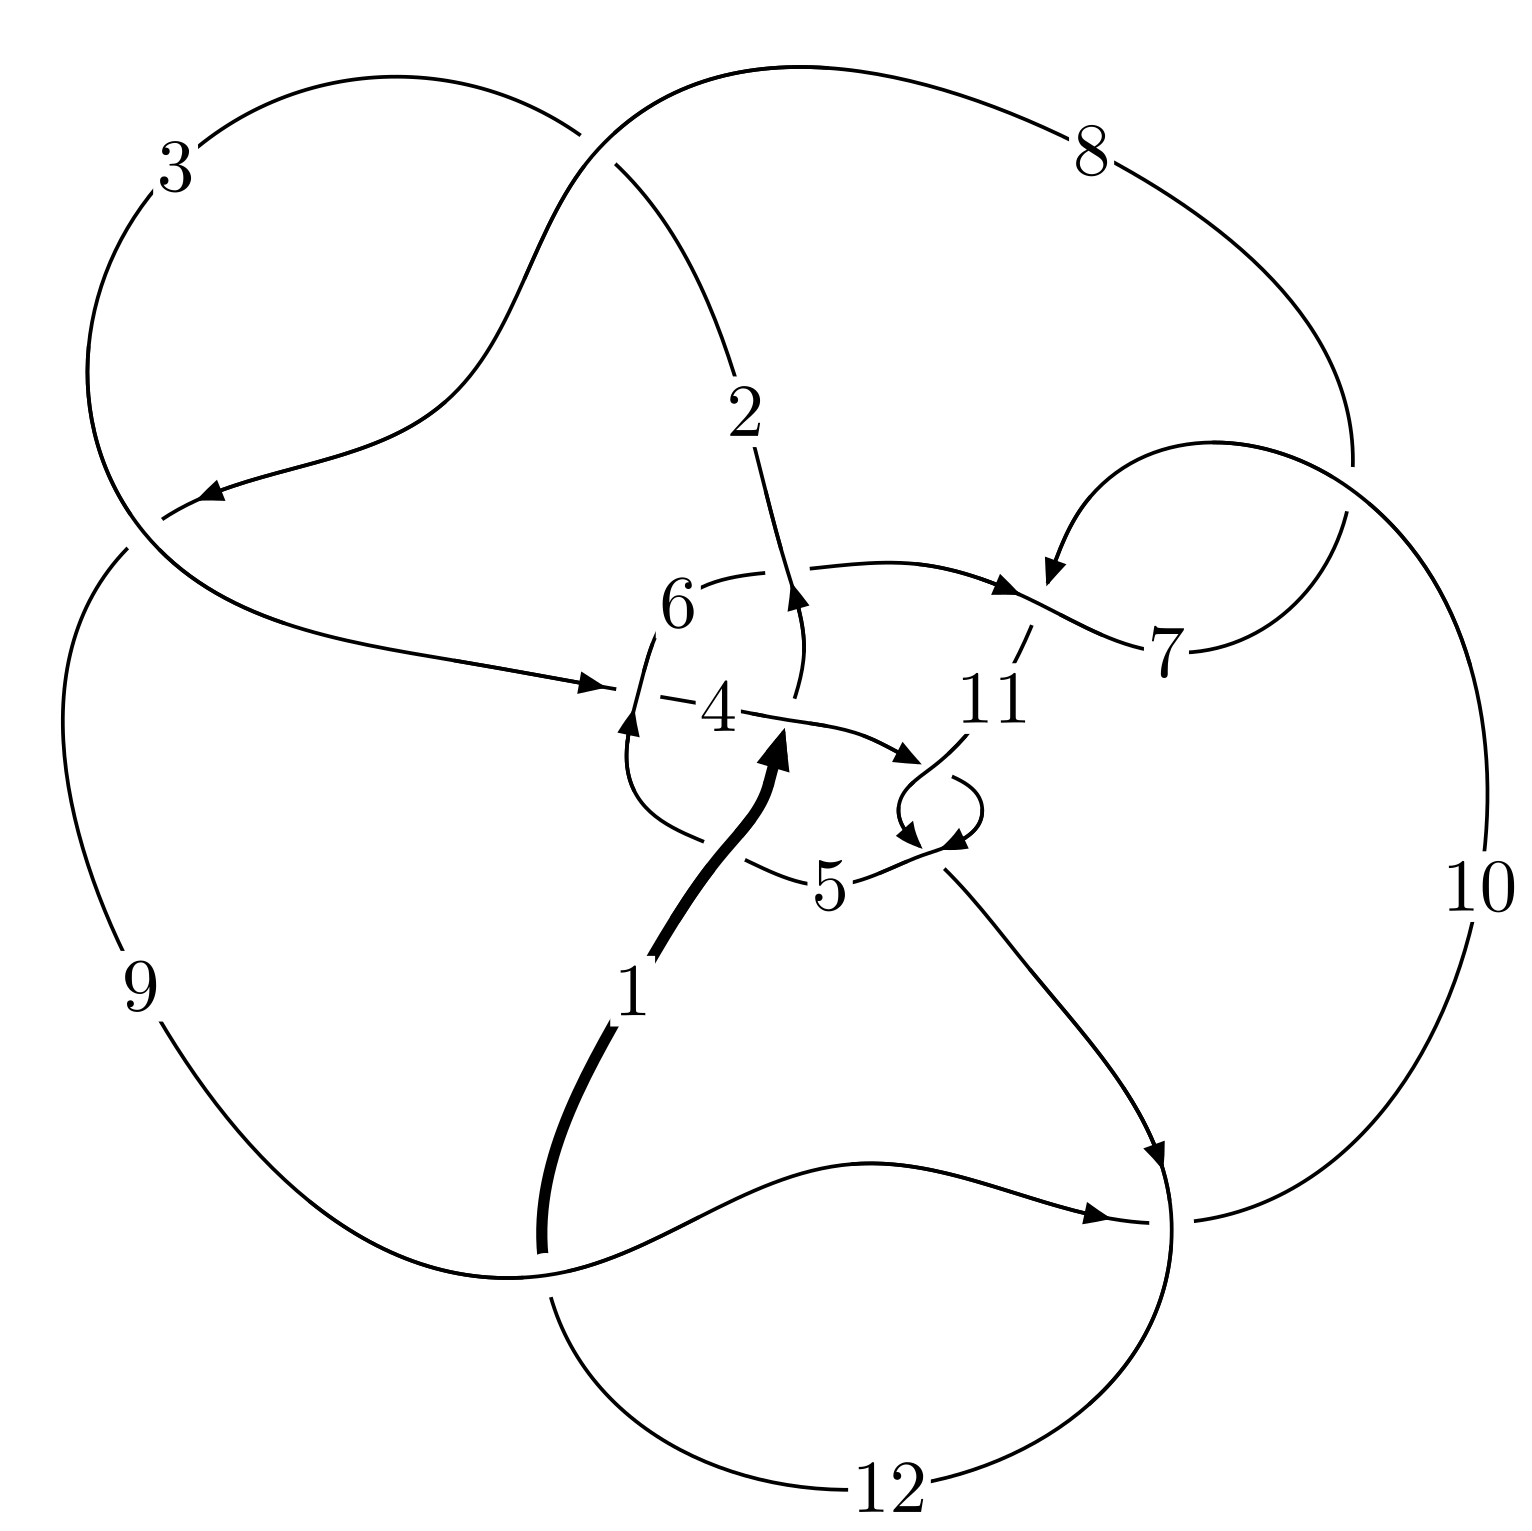
\includegraphics[width=112pt]{../../../GIT/diagram.site/Diagrams/png/1924_12a_1123.png}\\
\ \ \ A knot diagram\footnotemark}&
\allowdisplaybreaks
\textbf{Linearized knot diagam} \\
\cline{2-2}
 &
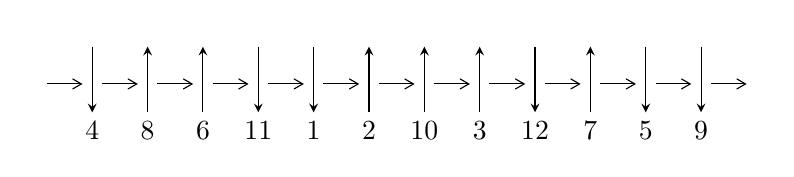
\begin{tikzpicture}[x=20pt, y=17pt]
	% nodes
	\node (C0) at (0, 0) {};
	\node (C1) at (1, 0) {};
	\node (C1U) at (1, +1) {};
	\node (C1D) at (1, -1) {4};

	\node (C2) at (2, 0) {};
	\node (C2U) at (2, +1) {};
	\node (C2D) at (2, -1) {8};

	\node (C3) at (3, 0) {};
	\node (C3U) at (3, +1) {};
	\node (C3D) at (3, -1) {6};

	\node (C4) at (4, 0) {};
	\node (C4U) at (4, +1) {};
	\node (C4D) at (4, -1) {11};

	\node (C5) at (5, 0) {};
	\node (C5U) at (5, +1) {};
	\node (C5D) at (5, -1) {1};

	\node (C6) at (6, 0) {};
	\node (C6U) at (6, +1) {};
	\node (C6D) at (6, -1) {2};

	\node (C7) at (7, 0) {};
	\node (C7U) at (7, +1) {};
	\node (C7D) at (7, -1) {10};

	\node (C8) at (8, 0) {};
	\node (C8U) at (8, +1) {};
	\node (C8D) at (8, -1) {3};

	\node (C9) at (9, 0) {};
	\node (C9U) at (9, +1) {};
	\node (C9D) at (9, -1) {12};

	\node (C10) at (10, 0) {};
	\node (C10U) at (10, +1) {};
	\node (C10D) at (10, -1) {7};

	\node (C11) at (11, 0) {};
	\node (C11U) at (11, +1) {};
	\node (C11D) at (11, -1) {5};

	\node (C12) at (12, 0) {};
	\node (C12U) at (12, +1) {};
	\node (C12D) at (12, -1) {9};
	\node (C13) at (13, 0) {};

	% arrows
	\draw[->,>={angle 60}]
	(C0) edge (C1) (C1) edge (C2) (C2) edge (C3) (C3) edge (C4) (C4) edge (C5) (C5) edge (C6) (C6) edge (C7) (C7) edge (C8) (C8) edge (C9) (C9) edge (C10) (C10) edge (C11) (C11) edge (C12) (C12) edge (C13) ;	\draw[->,>=stealth]
	(C1U) edge (C1D) (C2D) edge (C2U) (C3D) edge (C3U) (C4U) edge (C4D) (C5U) edge (C5D) (C6D) edge (C6U) (C7D) edge (C7U) (C8D) edge (C8U) (C9U) edge (C9D) (C10D) edge (C10U) (C11U) edge (C11D) (C12U) edge (C12D) ;
	\end{tikzpicture} \\
\hhline{~~} \\& 
\textbf{Solving Sequence} \\ \cline{2-2} 
 &
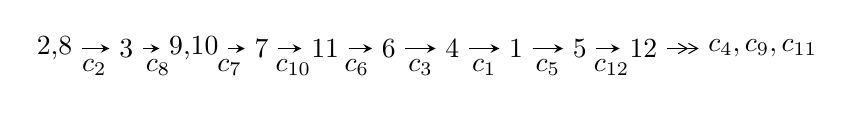
\begin{tikzpicture}[x=23pt, y=7pt]
	% node
	\node (A0) at (-1/8, 0) {2,8};
	\node (A1) at (1, 0) {3};
	\node (A2) at (33/16, 0) {9,10};
	\node (A3) at (25/8, 0) {7};
	\node (A4) at (33/8, 0) {11};
	\node (A5) at (41/8, 0) {6};
	\node (A6) at (49/8, 0) {4};
	\node (A7) at (57/8, 0) {1};
	\node (A8) at (65/8, 0) {5};
	\node (A9) at (73/8, 0) {12};
	\node (C1) at (1/2, -1) {$c_{2}$};
	\node (C2) at (3/2, -1) {$c_{8}$};
	\node (C3) at (21/8, -1) {$c_{7}$};
	\node (C4) at (29/8, -1) {$c_{10}$};
	\node (C5) at (37/8, -1) {$c_{6}$};
	\node (C6) at (45/8, -1) {$c_{3}$};
	\node (C7) at (53/8, -1) {$c_{1}$};
	\node (C8) at (61/8, -1) {$c_{5}$};
	\node (C9) at (69/8, -1) {$c_{12}$};
	\node (A10) at (11, 0) {$c_{4},c_{9},c_{11}$};

	% edge
	\draw[->,>=stealth]	
	(A0) edge (A1) (A1) edge (A2) (A2) edge (A3) (A3) edge (A4) (A4) edge (A5) (A5) edge (A6) (A6) edge (A7) (A7) edge (A8) (A8) edge (A9) ;
	\draw[->>,>={angle 60}]	
	(A9) edge (A10);
\end{tikzpicture} \\ 

\end{tabular} \\

\footnotetext{
The image of knot diagram is generated by the software ``\textbf{Draw programme}" developed by Andrew Bartholomew(\url{http://www.layer8.co.uk/maths/draw/index.htm\#Running-draw}), where we modified some parts for our purpose(\url{https://github.com/CATsTAILs/LinksPainter}).
}\phantom \\ \newline 
\centering \textbf{Ideals for irreducible components\footnotemark of $X_{\text{par}}$} 
 
\begin{align*}
I^u_{1}&=\langle 
-4.78617\times10^{1299} u^{183}+1.15209\times10^{1300} u^{182}+\cdots+3.43840\times10^{1301} b-4.60238\times10^{1305},\\
\phantom{I^u_{1}}&\phantom{= \langle  }-3.26625\times10^{1304} u^{183}+4.61565\times10^{1304} u^{182}+\cdots+3.04106\times10^{1306} a-2.55958\times10^{1310},\\
\phantom{I^u_{1}}&\phantom{= \langle  }u^{184}-3 u^{183}+\cdots-16532 u-707552\rangle \\
I^u_{2}&=\langle 
1.03964\times10^{80} u^{53}-1.41812\times10^{80} u^{52}+\cdots+1.18952\times10^{79} b-1.18053\times10^{81},\\
\phantom{I^u_{2}}&\phantom{= \langle  }-2.63097\times10^{81} u^{53}+5.32573\times10^{81} u^{52}+\cdots+7.61290\times10^{80} a-2.25246\times10^{82},\\
\phantom{I^u_{2}}&\phantom{= \langle  }u^{54}-2 u^{53}+\cdots+8 u+16\rangle \\
I^u_{3}&=\langle 
b,\;a+1,\;u+1\rangle \\
I^u_{4}&=\langle 
b-1,\;a,\;u-1\rangle \\
\\
I^v_{1}&=\langle 
a,\;b-1,\;v^2+v+1\rangle \\
\end{align*}
\raggedright * 5 irreducible components of $\dim_{\mathbb{C}}=0$, with total 242 representations.\\
\footnotetext{All coefficients of polynomials are rational numbers. But the coefficients are sometimes approximated in decimal forms when there is not enough margin.}
\newpage
\renewcommand{\arraystretch}{1}
\centering \section*{I. $I^u_{1}= \langle -4.79\times10^{1299} u^{183}+1.15\times10^{1300} u^{182}+\cdots+3.44\times10^{1301} b-4.60\times10^{1305},\;-3.27\times10^{1304} u^{183}+4.62\times10^{1304} u^{182}+\cdots+3.04\times10^{1306} a-2.56\times10^{1310},\;u^{184}-3 u^{183}+\cdots-16532 u-707552 \rangle$}
\flushleft \textbf{(i) Arc colorings}\\
\begin{tabular}{m{7pt} m{180pt} m{7pt} m{180pt} }
\flushright $a_{2}=$&$\begin{pmatrix}1\\0\end{pmatrix}$ \\
\flushright $a_{8}=$&$\begin{pmatrix}0\\u\end{pmatrix}$ \\
\flushright $a_{3}=$&$\begin{pmatrix}1\\- u^2\end{pmatrix}$ \\
\flushright $a_{9}=$&$\begin{pmatrix}u\\- u^3+u\end{pmatrix}$ \\
\flushright $a_{10}=$&$\begin{pmatrix}0.0107405 u^{183}-0.0151777 u^{182}+\cdots-3295.92 u+8416.72\\0.0139197 u^{183}-0.0335067 u^{182}+\cdots+19645.1 u+13385.2\end{pmatrix}$ \\
\flushright $a_{7}=$&$\begin{pmatrix}-0.00156752 u^{183}-0.00663758 u^{182}+\cdots+13051.4 u-4867.01\\0.00828057 u^{183}-0.0193654 u^{182}+\cdots-1932.56 u-1452.62\end{pmatrix}$ \\
\flushright $a_{11}=$&$\begin{pmatrix}-0.00127922 u^{183}+0.00655393 u^{182}+\cdots-25451.7 u-13831.3\\0.00717971 u^{183}-0.0194907 u^{182}+\cdots+20116.8 u+12169.8\end{pmatrix}$ \\
\flushright $a_{6}=$&$\begin{pmatrix}-0.00984809 u^{183}+0.0127279 u^{182}+\cdots+14983.9 u-3414.39\\0.00828057 u^{183}-0.0193654 u^{182}+\cdots-1932.56 u-1452.62\end{pmatrix}$ \\
\flushright $a_{4}=$&$\begin{pmatrix}0.0444811 u^{183}-0.115632 u^{182}+\cdots+48562.7 u+19528.8\\-0.0233998 u^{183}+0.0518711 u^{182}+\cdots-23431.8 u-19788.0\end{pmatrix}$ \\
\flushright $a_{1}=$&$\begin{pmatrix}0.0102005 u^{183}-0.0285372 u^{182}+\cdots+26048.7 u+11181.2\\-0.00245711 u^{183}+0.0108087 u^{182}+\cdots-15547.1 u-6467.78\end{pmatrix}$ \\
\flushright $a_{5}=$&$\begin{pmatrix}0.00849164 u^{183}-0.0254342 u^{182}+\cdots+23002.7 u+9454.99\\0.0314455 u^{183}-0.0656827 u^{182}+\cdots+25015.7 u+26410.8\end{pmatrix}$ \\
\flushright $a_{12}=$&$\begin{pmatrix}0.0115925 u^{183}-0.0268365 u^{182}+\cdots+16092.5 u+9751.18\\-0.00723329 u^{183}+0.0240324 u^{182}+\cdots-26585.3 u-12055.8\end{pmatrix}$\\&\end{tabular}
\flushleft \textbf{(ii) Obstruction class $= -1$}\\~\\
\flushleft \textbf{(iii) Cusp Shapes $= 0.189618 u^{183}-0.434216 u^{182}+\cdots+235912. u+190543.$}\\~\\
\newpage\renewcommand{\arraystretch}{1}
\flushleft \textbf{(iv) u-Polynomials at the component}\newline \\
\begin{tabular}{m{50pt}|m{274pt}}
Crossings & \hspace{64pt}u-Polynomials at each crossing \\
\hline $$\begin{aligned}c_{1}\end{aligned}$$&$\begin{aligned}
&u^{184}-24 u^{183}+\cdots-311 u+11
\end{aligned}$\\
\hline $$\begin{aligned}c_{2},c_{8}\end{aligned}$$&$\begin{aligned}
&u^{184}+3 u^{183}+\cdots+16532 u-707552
\end{aligned}$\\
\hline $$\begin{aligned}c_{3}\end{aligned}$$&$\begin{aligned}
&u^{184}+24 u^{183}+\cdots+311 u+11
\end{aligned}$\\
\hline $$\begin{aligned}c_{4},c_{11}\end{aligned}$$&$\begin{aligned}
&u^{184}-3 u^{183}+\cdots-16532 u-707552
\end{aligned}$\\
\hline $$\begin{aligned}c_{5}\end{aligned}$$&$\begin{aligned}
&u^{184}+3 u^{183}+\cdots-9319301 u-540938
\end{aligned}$\\
\hline $$\begin{aligned}c_{6}\end{aligned}$$&$\begin{aligned}
&u^{184}-3 u^{183}+\cdots+9319301 u-540938
\end{aligned}$\\
\hline $$\begin{aligned}c_{7},c_{10}\end{aligned}$$&$\begin{aligned}
&u^{184}+7 u^{183}+\cdots-35972490 u-2292697
\end{aligned}$\\
\hline $$\begin{aligned}c_{9},c_{12}\end{aligned}$$&$\begin{aligned}
&u^{184}-7 u^{183}+\cdots+35972490 u-2292697
\end{aligned}$\\
\hline
\end{tabular}\\~\\
\newpage\renewcommand{\arraystretch}{1}
\flushleft \textbf{(v) Riley Polynomials at the component}\newline \\
\begin{tabular}{m{50pt}|m{274pt}}
Crossings & \hspace{64pt}Riley Polynomials at each crossing \\
\hline $$\begin{aligned}c_{1},c_{3}\end{aligned}$$&$\begin{aligned}
&y^{184}-28 y^{183}+\cdots-4453 y+121
\end{aligned}$\\
\hline $$\begin{aligned}c_{2},c_{4},c_{8}\\c_{11}\end{aligned}$$&$\begin{aligned}
&y^{184}-123 y^{183}+\cdots-24369037776528 y+500629832704
\end{aligned}$\\
\hline $$\begin{aligned}c_{5},c_{6}\end{aligned}$$&$\begin{aligned}
&y^{184}+y^{183}+\cdots-44470573435141 y+292613919844
\end{aligned}$\\
\hline $$\begin{aligned}c_{7},c_{9},c_{10}\\c_{12}\end{aligned}$$&$\begin{aligned}
&y^{184}+87 y^{183}+\cdots+234883455129296 y+5256459533809
\end{aligned}$\\
\hline
\end{tabular}\\~\\
\newpage\flushleft \textbf{(vi) Complex Volumes and Cusp Shapes}
$$\begin{array}{c|c|c}  
\text{Solutions to }I^u_{1}& \I (\text{vol} + \sqrt{-1}CS) & \text{Cusp shape}\\
 \hline 
\begin{aligned}
u &= -0.985626\phantom{ +0.000000I} \\
a &= -0.759031\phantom{ +0.000000I} \\
b &= -0.0948487\phantom{ +0.000000I}\end{aligned}
 & \phantom{-}1.81166\phantom{ +0.000000I} & \phantom{-0.000000 } 0 \\ \hline\begin{aligned}
u &= -0.489911 + 0.901223 I \\
a &= -0.805025 + 0.681962 I \\
b &= -1.73608 + 0.05132 I\end{aligned}
 & -2.39271 + 3.21505 I & \phantom{-0.000000 } 0 \\ \hline\begin{aligned}
u &= -0.489911 - 0.901223 I \\
a &= -0.805025 - 0.681962 I \\
b &= -1.73608 - 0.05132 I\end{aligned}
 & -2.39271 - 3.21505 I & \phantom{-0.000000 } 0 \\ \hline\begin{aligned}
u &= \phantom{-}0.180610 + 1.011810 I \\
a &= \phantom{-}0.989830 + 0.658343 I \\
b &= \phantom{-}1.72828 - 0.03225 I\end{aligned}
 & -6.36700 - 8.19408 I & \phantom{-0.000000 } 0 \\ \hline\begin{aligned}
u &= \phantom{-}0.180610 - 1.011810 I \\
a &= \phantom{-}0.989830 - 0.658343 I \\
b &= \phantom{-}1.72828 + 0.03225 I\end{aligned}
 & -6.36700 + 8.19408 I & \phantom{-0.000000 } 0 \\ \hline\begin{aligned}
u &= -1.005260 + 0.230771 I \\
a &= -0.518244 + 0.930244 I \\
b &= -2.43905 + 0.47542 I\end{aligned}
 & -4.85131 - 2.59645 I & \phantom{-0.000000 } 0 \\ \hline\begin{aligned}
u &= -1.005260 - 0.230771 I \\
a &= -0.518244 - 0.930244 I \\
b &= -2.43905 - 0.47542 I\end{aligned}
 & -4.85131 + 2.59645 I & \phantom{-0.000000 } 0 \\ \hline\begin{aligned}
u &= -0.735384 + 0.613585 I \\
a &= -1.040240 + 0.411539 I \\
b &= -1.046980 - 0.525483 I\end{aligned}
 & \phantom{-}0.92484 - 2.06260 I & \phantom{-0.000000 } 0 \\ \hline\begin{aligned}
u &= -0.735384 - 0.613585 I \\
a &= -1.040240 - 0.411539 I \\
b &= -1.046980 + 0.525483 I\end{aligned}
 & \phantom{-}0.92484 + 2.06260 I & \phantom{-0.000000 } 0 \\ \hline\begin{aligned}
u &= -0.695315 + 0.782126 I \\
a &= -0.842301 + 0.964060 I \\
b &= -1.54098 + 0.12296 I\end{aligned}
 & -2.59109 + 2.11654 I & \phantom{-0.000000 } 0\\
 \hline 
 \end{array}$$\newpage$$\begin{array}{c|c|c}  
\text{Solutions to }I^u_{1}& \I (\text{vol} + \sqrt{-1}CS) & \text{Cusp shape}\\
 \hline 
\begin{aligned}
u &= -0.695315 - 0.782126 I \\
a &= -0.842301 - 0.964060 I \\
b &= -1.54098 - 0.12296 I\end{aligned}
 & -2.59109 - 2.11654 I & \phantom{-0.000000 } 0 \\ \hline\begin{aligned}
u &= \phantom{-}0.798329 + 0.499550 I \\
a &= \phantom{-}0.765281 + 0.620111 I \\
b &= \phantom{-}0.84266 - 1.52141 I\end{aligned}
 & -1.93610 + 3.47025 I & \phantom{-0.000000 } 0 \\ \hline\begin{aligned}
u &= \phantom{-}0.798329 - 0.499550 I \\
a &= \phantom{-}0.765281 - 0.620111 I \\
b &= \phantom{-}0.84266 + 1.52141 I\end{aligned}
 & -1.93610 - 3.47025 I & \phantom{-0.000000 } 0 \\ \hline\begin{aligned}
u &= \phantom{-}0.704438 + 0.615542 I \\
a &= \phantom{-}1.27157 + 1.33467 I \\
b &= \phantom{-}1.034560 - 0.424468 I\end{aligned}
 & -5.60582 + 8.27968 I & \phantom{-0.000000 } 0 \\ \hline\begin{aligned}
u &= \phantom{-}0.704438 - 0.615542 I \\
a &= \phantom{-}1.27157 - 1.33467 I \\
b &= \phantom{-}1.034560 + 0.424468 I\end{aligned}
 & -5.60582 - 8.27968 I & \phantom{-0.000000 } 0 \\ \hline\begin{aligned}
u &= -0.804895 + 0.702904 I \\
a &= \phantom{-}0.560383 - 0.038561 I \\
b &= \phantom{-}1.54722 + 1.16442 I\end{aligned}
 & \phantom{-}2.92723 - 2.77066 I & \phantom{-0.000000 } 0 \\ \hline\begin{aligned}
u &= -0.804895 - 0.702904 I \\
a &= \phantom{-}0.560383 + 0.038561 I \\
b &= \phantom{-}1.54722 - 1.16442 I\end{aligned}
 & \phantom{-}2.92723 + 2.77066 I & \phantom{-0.000000 } 0 \\ \hline\begin{aligned}
u &= \phantom{-}0.926286 + 0.014329 I \\
a &= -0.821084 + 0.987438 I \\
b &= -1.53496 - 0.43276 I\end{aligned}
 & \phantom{-}2.26240 - 3.62583 I & \phantom{-0.000000 } 0 \\ \hline\begin{aligned}
u &= \phantom{-}0.926286 - 0.014329 I \\
a &= -0.821084 - 0.987438 I \\
b &= -1.53496 + 0.43276 I\end{aligned}
 & \phantom{-}2.26240 + 3.62583 I & \phantom{-0.000000 } 0 \\ \hline\begin{aligned}
u &= -0.902918 + 0.206522 I \\
a &= \phantom{-}0.60340 + 1.46916 I \\
b &= \phantom{-}0.662486 - 0.622978 I\end{aligned}
 & \phantom{-}1.38239 - 3.23354 I & \phantom{-0.000000 } 0\\
 \hline 
 \end{array}$$\newpage$$\begin{array}{c|c|c}  
\text{Solutions to }I^u_{1}& \I (\text{vol} + \sqrt{-1}CS) & \text{Cusp shape}\\
 \hline 
\begin{aligned}
u &= -0.902918 - 0.206522 I \\
a &= \phantom{-}0.60340 - 1.46916 I \\
b &= \phantom{-}0.662486 + 0.622978 I\end{aligned}
 & \phantom{-}1.38239 + 3.23354 I & \phantom{-0.000000 } 0 \\ \hline\begin{aligned}
u &= \phantom{-}0.892620 + 0.236399 I \\
a &= -0.92437 - 1.07973 I \\
b &= -1.385630 - 0.021065 I\end{aligned}
 & -6.00362 - 0.84358 I & \phantom{-0.000000 } 0 \\ \hline\begin{aligned}
u &= \phantom{-}0.892620 - 0.236399 I \\
a &= -0.92437 + 1.07973 I \\
b &= -1.385630 + 0.021065 I\end{aligned}
 & -6.00362 + 0.84358 I & \phantom{-0.000000 } 0 \\ \hline\begin{aligned}
u &= \phantom{-}1.022330 + 0.356426 I \\
a &= -1.111570 + 0.780898 I \\
b &= -0.606798 + 0.620247 I\end{aligned}
 & \phantom{-}4.85131 + 2.59645 I & \phantom{-0.000000 } 0 \\ \hline\begin{aligned}
u &= \phantom{-}1.022330 - 0.356426 I \\
a &= -1.111570 - 0.780898 I \\
b &= -0.606798 - 0.620247 I\end{aligned}
 & \phantom{-}4.85131 - 2.59645 I & \phantom{-0.000000 } 0 \\ \hline\begin{aligned}
u &= -1.074620 + 0.166743 I \\
a &= \phantom{-}1.93510 + 0.18775 I \\
b &= \phantom{-}0.413987 - 0.051585 I\end{aligned}
 & \phantom{-}2.01208 - 2.54820 I & \phantom{-0.000000 } 0 \\ \hline\begin{aligned}
u &= -1.074620 - 0.166743 I \\
a &= \phantom{-}1.93510 - 0.18775 I \\
b &= \phantom{-}0.413987 + 0.051585 I\end{aligned}
 & \phantom{-}2.01208 + 2.54820 I & \phantom{-0.000000 } 0 \\ \hline\begin{aligned}
u &= \phantom{-}0.802134 + 0.421950 I \\
a &= \phantom{-}0.789056 + 0.986182 I \\
b &= \phantom{-}1.21198 - 1.39302 I\end{aligned}
 & -1.97744 + 2.96340 I & \phantom{-0.000000 } 0 \\ \hline\begin{aligned}
u &= \phantom{-}0.802134 - 0.421950 I \\
a &= \phantom{-}0.789056 - 0.986182 I \\
b &= \phantom{-}1.21198 + 1.39302 I\end{aligned}
 & -1.97744 - 2.96340 I & \phantom{-0.000000 } 0 \\ \hline\begin{aligned}
u &= -0.048778 + 0.901957 I \\
a &= \phantom{-}0.250954 - 0.600412 I \\
b &= \phantom{-}1.087460 + 0.094327 I\end{aligned}
 & \phantom{-}2.39271 - 3.21505 I & \phantom{-0.000000 } 0\\
 \hline 
 \end{array}$$\newpage$$\begin{array}{c|c|c}  
\text{Solutions to }I^u_{1}& \I (\text{vol} + \sqrt{-1}CS) & \text{Cusp shape}\\
 \hline 
\begin{aligned}
u &= -0.048778 - 0.901957 I \\
a &= \phantom{-}0.250954 + 0.600412 I \\
b &= \phantom{-}1.087460 - 0.094327 I\end{aligned}
 & \phantom{-}2.39271 + 3.21505 I & \phantom{-0.000000 } 0 \\ \hline\begin{aligned}
u &= -0.026037 + 0.902429 I \\
a &= -1.093070 - 0.695436 I \\
b &= -1.302130 + 0.025427 I\end{aligned}
 & \phantom{-}0.85382 - 2.87397 I & \phantom{-0.000000 } 0 \\ \hline\begin{aligned}
u &= -0.026037 - 0.902429 I \\
a &= -1.093070 + 0.695436 I \\
b &= -1.302130 - 0.025427 I\end{aligned}
 & \phantom{-}0.85382 + 2.87397 I & \phantom{-0.000000 } 0 \\ \hline\begin{aligned}
u &= -0.276070 + 0.858657 I \\
a &= -0.413887 - 1.076220 I \\
b &= -0.933141 - 0.154161 I\end{aligned}
 & \phantom{-}0.12293 + 8.60047 I & \phantom{-0.000000 } 0 \\ \hline\begin{aligned}
u &= -0.276070 - 0.858657 I \\
a &= -0.413887 + 1.076220 I \\
b &= -0.933141 + 0.154161 I\end{aligned}
 & \phantom{-}0.12293 - 8.60047 I & \phantom{-0.000000 } 0 \\ \hline\begin{aligned}
u &= -0.845699 + 0.295331 I \\
a &= -1.354790 + 0.269684 I \\
b &= -0.437180 + 0.241808 I\end{aligned}
 & \phantom{-}1.39201 + 0.99343 I & \phantom{-0.000000 } 0 \\ \hline\begin{aligned}
u &= -0.845699 - 0.295331 I \\
a &= -1.354790 - 0.269684 I \\
b &= -0.437180 - 0.241808 I\end{aligned}
 & \phantom{-}1.39201 - 0.99343 I & \phantom{-0.000000 } 0 \\ \hline\begin{aligned}
u &= \phantom{-}1.087200 + 0.302579 I \\
a &= -0.679623 - 0.666667 I \\
b &= -1.87872 - 0.32585 I\end{aligned}
 & \phantom{-}1.43596 + 5.96515 I & \phantom{-0.000000 } 0 \\ \hline\begin{aligned}
u &= \phantom{-}1.087200 - 0.302579 I \\
a &= -0.679623 + 0.666667 I \\
b &= -1.87872 + 0.32585 I\end{aligned}
 & \phantom{-}1.43596 - 5.96515 I & \phantom{-0.000000 } 0 \\ \hline\begin{aligned}
u &= -0.678508 + 0.913644 I \\
a &= -0.704081 + 0.788464 I \\
b &= -0.845690 - 0.370506 I\end{aligned}
 & -2.26240 - 3.62583 I & \phantom{-0.000000 } 0\\
 \hline 
 \end{array}$$\newpage$$\begin{array}{c|c|c}  
\text{Solutions to }I^u_{1}& \I (\text{vol} + \sqrt{-1}CS) & \text{Cusp shape}\\
 \hline 
\begin{aligned}
u &= -0.678508 - 0.913644 I \\
a &= -0.704081 - 0.788464 I \\
b &= -0.845690 + 0.370506 I\end{aligned}
 & -2.26240 + 3.62583 I & \phantom{-0.000000 } 0 \\ \hline\begin{aligned}
u &= \phantom{-}0.685478 + 0.514961 I \\
a &= \phantom{-}0.574553 + 0.851611 I \\
b &= \phantom{-}1.73144 - 0.28433 I\end{aligned}
 & -2.36266 + 1.01498 I & \phantom{-0.000000 } 0 \\ \hline\begin{aligned}
u &= \phantom{-}0.685478 - 0.514961 I \\
a &= \phantom{-}0.574553 - 0.851611 I \\
b &= \phantom{-}1.73144 + 0.28433 I\end{aligned}
 & -2.36266 - 1.01498 I & \phantom{-0.000000 } 0 \\ \hline\begin{aligned}
u &= -0.825897 + 0.198082 I \\
a &= -2.10285 - 0.24188 I \\
b &= -0.373539 + 0.076539 I\end{aligned}
 & \phantom{-}1.37257 + 1.21094 I & \phantom{-0.000000 } 0 \\ \hline\begin{aligned}
u &= -0.825897 - 0.198082 I \\
a &= -2.10285 + 0.24188 I \\
b &= -0.373539 - 0.076539 I\end{aligned}
 & \phantom{-}1.37257 - 1.21094 I & \phantom{-0.000000 } 0 \\ \hline\begin{aligned}
u &= \phantom{-}0.804476 + 0.269267 I \\
a &= -0.36857 - 1.72115 I \\
b &= -0.620916 + 0.712355 I\end{aligned}
 & -6.16249 + 3.26145 I & \phantom{-0.000000 } 0 \\ \hline\begin{aligned}
u &= \phantom{-}0.804476 - 0.269267 I \\
a &= -0.36857 + 1.72115 I \\
b &= -0.620916 - 0.712355 I\end{aligned}
 & -6.16249 - 3.26145 I & \phantom{-0.000000 } 0 \\ \hline\begin{aligned}
u &= \phantom{-}0.840768 + 0.080079 I \\
a &= \phantom{-}0.371275 + 0.852191 I \\
b &= \phantom{-}3.02870 - 0.28547 I\end{aligned}
 & -3.64266 - 0.21557 I & \phantom{-0.000000 } 0 \\ \hline\begin{aligned}
u &= \phantom{-}0.840768 - 0.080079 I \\
a &= \phantom{-}0.371275 - 0.852191 I \\
b &= \phantom{-}3.02870 + 0.28547 I\end{aligned}
 & -3.64266 + 0.21557 I & \phantom{-0.000000 } 0 \\ \hline\begin{aligned}
u &= \phantom{-}1.070720 + 0.458245 I \\
a &= -0.446676 - 0.312714 I \\
b &= -1.79888 - 0.47416 I\end{aligned}
 & \phantom{-}1.19256 + 6.47923 I & \phantom{-0.000000 } 0\\
 \hline 
 \end{array}$$\newpage$$\begin{array}{c|c|c}  
\text{Solutions to }I^u_{1}& \I (\text{vol} + \sqrt{-1}CS) & \text{Cusp shape}\\
 \hline 
\begin{aligned}
u &= \phantom{-}1.070720 - 0.458245 I \\
a &= -0.446676 + 0.312714 I \\
b &= -1.79888 + 0.47416 I\end{aligned}
 & \phantom{-}1.19256 - 6.47923 I & \phantom{-0.000000 } 0 \\ \hline\begin{aligned}
u &= \phantom{-}1.072110 + 0.475562 I \\
a &= \phantom{-}0.983675 + 0.735838 I \\
b &= \phantom{-}1.31882 - 0.65322 I\end{aligned}
 & -2.17391 + 6.57641 I & \phantom{-0.000000 } 0 \\ \hline\begin{aligned}
u &= \phantom{-}1.072110 - 0.475562 I \\
a &= \phantom{-}0.983675 - 0.735838 I \\
b &= \phantom{-}1.31882 + 0.65322 I\end{aligned}
 & -2.17391 - 6.57641 I & \phantom{-0.000000 } 0 \\ \hline\begin{aligned}
u &= \phantom{-}1.149500 + 0.237840 I \\
a &= \phantom{-}0.791790 - 0.107984 I \\
b &= \phantom{-}0.091517 - 0.162488 I\end{aligned}
 & \phantom{-}3.92123 + 3.79257 I & \phantom{-0.000000 } 0 \\ \hline\begin{aligned}
u &= \phantom{-}1.149500 - 0.237840 I \\
a &= \phantom{-}0.791790 + 0.107984 I \\
b &= \phantom{-}0.091517 + 0.162488 I\end{aligned}
 & \phantom{-}3.92123 - 3.79257 I & \phantom{-0.000000 } 0 \\ \hline\begin{aligned}
u &= -0.042621 + 0.824732 I \\
a &= -1.359300 + 0.185818 I \\
b &= -1.70822 - 0.28360 I\end{aligned}
 & -8.32646 - 1.63543 I & \phantom{-0.000000 } 0 \\ \hline\begin{aligned}
u &= -0.042621 - 0.824732 I \\
a &= -1.359300 - 0.185818 I \\
b &= -1.70822 + 0.28360 I\end{aligned}
 & -8.32646 + 1.63543 I & \phantom{-0.000000 } 0 \\ \hline\begin{aligned}
u &= -0.924643 + 0.730244 I \\
a &= -0.504614 + 0.805299 I \\
b &= -1.61874 + 0.10520 I\end{aligned}
 & -2.92723 + 2.77066 I & \phantom{-0.000000 } 0 \\ \hline\begin{aligned}
u &= -0.924643 - 0.730244 I \\
a &= -0.504614 - 0.805299 I \\
b &= -1.61874 - 0.10520 I\end{aligned}
 & -2.92723 - 2.77066 I & \phantom{-0.000000 } 0 \\ \hline\begin{aligned}
u &= \phantom{-}0.921134 + 0.736510 I \\
a &= \phantom{-}1.031950 + 0.808342 I \\
b &= \phantom{-}1.51095 + 0.03229 I\end{aligned}
 & -5.01958 - 3.02663 I & \phantom{-0.000000 } 0\\
 \hline 
 \end{array}$$\newpage$$\begin{array}{c|c|c}  
\text{Solutions to }I^u_{1}& \I (\text{vol} + \sqrt{-1}CS) & \text{Cusp shape}\\
 \hline 
\begin{aligned}
u &= \phantom{-}0.921134 - 0.736510 I \\
a &= \phantom{-}1.031950 - 0.808342 I \\
b &= \phantom{-}1.51095 - 0.03229 I\end{aligned}
 & -5.01958 + 3.02663 I & \phantom{-0.000000 } 0 \\ \hline\begin{aligned}
u &= -1.165720 + 0.181056 I \\
a &= \phantom{-}1.007540 - 0.684382 I \\
b &= \phantom{-}0.767129 - 0.055654 I\end{aligned}
 & \phantom{-}2.34591 - 2.81285 I & \phantom{-0.000000 } 0 \\ \hline\begin{aligned}
u &= -1.165720 - 0.181056 I \\
a &= \phantom{-}1.007540 + 0.684382 I \\
b &= \phantom{-}0.767129 + 0.055654 I\end{aligned}
 & \phantom{-}2.34591 + 2.81285 I & \phantom{-0.000000 } 0 \\ \hline\begin{aligned}
u &= \phantom{-}0.643907 + 0.991431 I \\
a &= -0.204606 - 0.802795 I \\
b &= -0.404066 + 0.728819 I\end{aligned}
 & -0.33746 - 1.88661 I & \phantom{-0.000000 } 0 \\ \hline\begin{aligned}
u &= \phantom{-}0.643907 - 0.991431 I \\
a &= -0.204606 + 0.802795 I \\
b &= -0.404066 - 0.728819 I\end{aligned}
 & -0.33746 + 1.88661 I & \phantom{-0.000000 } 0 \\ \hline\begin{aligned}
u &= \phantom{-}0.621279 + 0.529397 I \\
a &= \phantom{-}1.60176 + 0.65665 I \\
b &= \phantom{-}1.41036 - 0.66133 I\end{aligned}
 & -1.19256 + 6.47923 I & \phantom{-0.000000 } 0 \\ \hline\begin{aligned}
u &= \phantom{-}0.621279 - 0.529397 I \\
a &= \phantom{-}1.60176 - 0.65665 I \\
b &= \phantom{-}1.41036 + 0.66133 I\end{aligned}
 & -1.19256 - 6.47923 I & \phantom{-0.000000 } 0 \\ \hline\begin{aligned}
u &= -0.784895 + 0.200538 I \\
a &= -0.25570 + 1.53212 I \\
b &= -1.34200 - 1.82242 I\end{aligned}
 & -5.62429 + 0.58912 I & \phantom{-0.000000 } 0 \\ \hline\begin{aligned}
u &= -0.784895 - 0.200538 I \\
a &= -0.25570 - 1.53212 I \\
b &= -1.34200 + 1.82242 I\end{aligned}
 & -5.62429 - 0.58912 I & \phantom{-0.000000 } 0 \\ \hline\begin{aligned}
u &= -0.968502 + 0.692552 I \\
a &= -1.124240 + 0.794564 I \\
b &= -1.56155 - 0.91365 I\end{aligned}
 & -1.79220 - 7.65639 I & \phantom{-0.000000 } 0\\
 \hline 
 \end{array}$$\newpage$$\begin{array}{c|c|c}  
\text{Solutions to }I^u_{1}& \I (\text{vol} + \sqrt{-1}CS) & \text{Cusp shape}\\
 \hline 
\begin{aligned}
u &= -0.968502 - 0.692552 I \\
a &= -1.124240 - 0.794564 I \\
b &= -1.56155 + 0.91365 I\end{aligned}
 & -1.79220 + 7.65639 I & \phantom{-0.000000 } 0 \\ \hline\begin{aligned}
u &= -1.185070 + 0.256522 I \\
a &= \phantom{-}0.408279 - 0.757112 I \\
b &= \phantom{-}1.85872 + 1.73919 I\end{aligned}
 & \phantom{-}5.01958 - 3.02663 I & \phantom{-0.000000 } 0 \\ \hline\begin{aligned}
u &= -1.185070 - 0.256522 I \\
a &= \phantom{-}0.408279 + 0.757112 I \\
b &= \phantom{-}1.85872 - 1.73919 I\end{aligned}
 & \phantom{-}5.01958 + 3.02663 I & \phantom{-0.000000 } 0 \\ \hline\begin{aligned}
u &= -0.778837 + 0.096749 I \\
a &= \phantom{-}0.304418 + 0.830487 I \\
b &= \phantom{-}2.26561 + 0.08753 I\end{aligned}
 & \phantom{-}2.59109 - 2.11654 I & \phantom{-0.000000 } 0 \\ \hline\begin{aligned}
u &= -0.778837 - 0.096749 I \\
a &= \phantom{-}0.304418 - 0.830487 I \\
b &= \phantom{-}2.26561 - 0.08753 I\end{aligned}
 & \phantom{-}2.59109 + 2.11654 I & \phantom{-0.000000 } 0 \\ \hline\begin{aligned}
u &= \phantom{-}0.762096 + 0.147835 I \\
a &= \phantom{-}1.04721 - 0.96385 I \\
b &= -0.484359 + 0.173774 I\end{aligned}
 & \phantom{-}1.93610 - 3.47025 I & \phantom{-0.000000 } 0 \\ \hline\begin{aligned}
u &= \phantom{-}0.762096 - 0.147835 I \\
a &= \phantom{-}1.04721 + 0.96385 I \\
b &= -0.484359 - 0.173774 I\end{aligned}
 & \phantom{-}1.93610 + 3.47025 I & \phantom{-0.000000 } 0 \\ \hline\begin{aligned}
u &= \phantom{-}0.088281 + 0.769342 I \\
a &= \phantom{-}0.257711 + 0.884805 I \\
b &= \phantom{-}0.502611 + 0.230620 I\end{aligned}
 & -3.92123 + 3.79257 I & \phantom{-0.000000 } 0 \\ \hline\begin{aligned}
u &= \phantom{-}0.088281 - 0.769342 I \\
a &= \phantom{-}0.257711 - 0.884805 I \\
b &= \phantom{-}0.502611 - 0.230620 I\end{aligned}
 & -3.92123 - 3.79257 I & \phantom{-0.000000 } 0 \\ \hline\begin{aligned}
u &= -0.749260 + 0.188813 I \\
a &= \phantom{-}1.36145 - 0.76811 I \\
b &= \phantom{-}1.43287 - 0.08567 I\end{aligned}
 & -4.48506 - 6.68699 I & \phantom{-0.000000 } 0\\
 \hline 
 \end{array}$$\newpage$$\begin{array}{c|c|c}  
\text{Solutions to }I^u_{1}& \I (\text{vol} + \sqrt{-1}CS) & \text{Cusp shape}\\
 \hline 
\begin{aligned}
u &= -0.749260 - 0.188813 I \\
a &= \phantom{-}1.36145 + 0.76811 I \\
b &= \phantom{-}1.43287 + 0.08567 I\end{aligned}
 & -4.48506 + 6.68699 I & \phantom{-0.000000 } 0 \\ \hline\begin{aligned}
u &= -1.189610 + 0.310866 I \\
a &= \phantom{-}0.557553 - 0.902645 I \\
b &= \phantom{-}1.99711 - 0.61768 I\end{aligned}
 & -1.42220 - 10.12460 I & \phantom{-0.000000 } 0 \\ \hline\begin{aligned}
u &= -1.189610 - 0.310866 I \\
a &= \phantom{-}0.557553 + 0.902645 I \\
b &= \phantom{-}1.99711 + 0.61768 I\end{aligned}
 & -1.42220 + 10.12460 I & \phantom{-0.000000 } 0 \\ \hline\begin{aligned}
u &= \phantom{-}0.717969 + 0.275469 I \\
a &= \phantom{-}1.85236 - 0.79530 I \\
b &= \phantom{-}0.289215 - 0.504753 I\end{aligned}
 & \phantom{-}3.64266 + 0.21557 I & \phantom{-0.000000 } 0 \\ \hline\begin{aligned}
u &= \phantom{-}0.717969 - 0.275469 I \\
a &= \phantom{-}1.85236 + 0.79530 I \\
b &= \phantom{-}0.289215 + 0.504753 I\end{aligned}
 & \phantom{-}3.64266 - 0.21557 I & \phantom{-0.000000 } 0 \\ \hline\begin{aligned}
u &= -1.176010 + 0.385573 I \\
a &= \phantom{-}0.781375 + 0.845819 I \\
b &= \phantom{-}0.315439 + 0.698136 I\end{aligned}
 & \phantom{-}5.62429 - 0.58912 I & \phantom{-0.000000 } 0 \\ \hline\begin{aligned}
u &= -1.176010 - 0.385573 I \\
a &= \phantom{-}0.781375 - 0.845819 I \\
b &= \phantom{-}0.315439 - 0.698136 I\end{aligned}
 & \phantom{-}5.62429 + 0.58912 I & \phantom{-0.000000 } 0 \\ \hline\begin{aligned}
u &= \phantom{-}0.737580 + 0.170365 I \\
a &= \phantom{-}0.034747 + 0.642731 I \\
b &= -3.02888 - 1.21694 I\end{aligned}
 & \phantom{-}1.79220 + 7.65639 I & \phantom{-0.000000 } 0 \\ \hline\begin{aligned}
u &= \phantom{-}0.737580 - 0.170365 I \\
a &= \phantom{-}0.034747 - 0.642731 I \\
b &= -3.02888 + 1.21694 I\end{aligned}
 & \phantom{-}1.79220 - 7.65639 I & \phantom{-0.000000 } 0 \\ \hline\begin{aligned}
u &= -1.168710 + 0.469901 I \\
a &= \phantom{-}0.951405 - 0.803807 I \\
b &= \phantom{-}2.06525 + 0.87580 I\end{aligned}
 & \phantom{-}1.42220 - 10.12460 I & \phantom{-0.000000 } 0\\
 \hline 
 \end{array}$$\newpage$$\begin{array}{c|c|c}  
\text{Solutions to }I^u_{1}& \I (\text{vol} + \sqrt{-1}CS) & \text{Cusp shape}\\
 \hline 
\begin{aligned}
u &= -1.168710 - 0.469901 I \\
a &= \phantom{-}0.951405 + 0.803807 I \\
b &= \phantom{-}2.06525 - 0.87580 I\end{aligned}
 & \phantom{-}1.42220 + 10.12460 I & \phantom{-0.000000 } 0 \\ \hline\begin{aligned}
u &= -0.721684 + 0.046606 I \\
a &= -1.19431 + 1.73762 I \\
b &= -0.500365 - 0.556419 I\end{aligned}
 & \phantom{-}0.33746 - 1.88661 I & \phantom{-0.000000 } 0 \\ \hline\begin{aligned}
u &= -0.721684 - 0.046606 I \\
a &= -1.19431 - 1.73762 I \\
b &= -0.500365 + 0.556419 I\end{aligned}
 & \phantom{-}0.33746 + 1.88661 I & \phantom{-0.000000 } 0 \\ \hline\begin{aligned}
u &= -1.226210 + 0.402234 I \\
a &= -0.697110 - 0.456871 I \\
b &= -0.187976 - 0.345164 I\end{aligned}
 & \phantom{-0.000000 } -7.92691 I & \phantom{-0.000000 } 0 \\ \hline\begin{aligned}
u &= -1.226210 - 0.402234 I \\
a &= -0.697110 + 0.456871 I \\
b &= -0.187976 + 0.345164 I\end{aligned}
 & \phantom{-0.000000 -}7.92691 I & \phantom{-0.000000 } 0 \\ \hline\begin{aligned}
u &= -1.162010 + 0.566310 I \\
a &= -0.745071 + 0.716572 I \\
b &= -1.70951 - 1.28188 I\end{aligned}
 & -0.12293 - 8.60047 I & \phantom{-0.000000 } 0 \\ \hline\begin{aligned}
u &= -1.162010 - 0.566310 I \\
a &= -0.745071 - 0.716572 I \\
b &= -1.70951 + 1.28188 I\end{aligned}
 & -0.12293 + 8.60047 I & \phantom{-0.000000 } 0 \\ \hline\begin{aligned}
u &= -1.225820 + 0.422841 I \\
a &= \phantom{-}0.124919 - 0.619537 I \\
b &= \phantom{-}1.45694 - 0.36010 I\end{aligned}
 & -1.01899 - 1.60810 I & \phantom{-0.000000 } 0 \\ \hline\begin{aligned}
u &= -1.225820 - 0.422841 I \\
a &= \phantom{-}0.124919 + 0.619537 I \\
b &= \phantom{-}1.45694 + 0.36010 I\end{aligned}
 & -1.01899 + 1.60810 I & \phantom{-0.000000 } 0 \\ \hline\begin{aligned}
u &= -0.332867 + 0.597578 I \\
a &= -2.06363 + 0.44611 I \\
b &= -0.929860 - 0.890913 I\end{aligned}
 & -4.26869 - 7.87376 I & \phantom{-0.000000 } 0\\
 \hline 
 \end{array}$$\newpage$$\begin{array}{c|c|c}  
\text{Solutions to }I^u_{1}& \I (\text{vol} + \sqrt{-1}CS) & \text{Cusp shape}\\
 \hline 
\begin{aligned}
u &= -0.332867 - 0.597578 I \\
a &= -2.06363 - 0.44611 I \\
b &= -0.929860 + 0.890913 I\end{aligned}
 & -4.26869 + 7.87376 I & \phantom{-0.000000 } 0 \\ \hline\begin{aligned}
u &= \phantom{-}0.110455 + 0.672101 I \\
a &= \phantom{-}1.60907 + 0.72067 I \\
b &= \phantom{-}0.875021 + 0.469568 I\end{aligned}
 & -4.78758 - 2.34370 I & \phantom{-0.000000 } 0 \\ \hline\begin{aligned}
u &= \phantom{-}0.110455 - 0.672101 I \\
a &= \phantom{-}1.60907 - 0.72067 I \\
b &= \phantom{-}0.875021 - 0.469568 I\end{aligned}
 & -4.78758 + 2.34370 I & \phantom{-0.000000 } 0 \\ \hline\begin{aligned}
u &= \phantom{-}1.019410 + 0.843827 I \\
a &= \phantom{-}0.609046 + 0.245167 I \\
b &= \phantom{-}1.90886 - 0.46068 I\end{aligned}
 & -1.39201 + 0.99343 I & \phantom{-0.000000 } 0 \\ \hline\begin{aligned}
u &= \phantom{-}1.019410 - 0.843827 I \\
a &= \phantom{-}0.609046 - 0.245167 I \\
b &= \phantom{-}1.90886 + 0.46068 I\end{aligned}
 & -1.39201 - 0.99343 I & \phantom{-0.000000 } 0 \\ \hline\begin{aligned}
u &= \phantom{-}1.214970 + 0.528259 I \\
a &= -0.896657 - 0.451155 I \\
b &= -2.14826 + 1.05482 I\end{aligned}
 & \phantom{-}4.41467 + 7.92340 I & \phantom{-0.000000 } 0 \\ \hline\begin{aligned}
u &= \phantom{-}1.214970 - 0.528259 I \\
a &= -0.896657 + 0.451155 I \\
b &= -2.14826 - 1.05482 I\end{aligned}
 & \phantom{-}4.41467 - 7.92340 I & \phantom{-0.000000 } 0 \\ \hline\begin{aligned}
u &= \phantom{-}0.303671 + 0.596367 I \\
a &= -0.529378 - 0.399748 I \\
b &= \phantom{-}0.048285 + 1.169730 I\end{aligned}
 & -0.92484 - 2.06260 I & \phantom{-0.000000 } 0 \\ \hline\begin{aligned}
u &= \phantom{-}0.303671 - 0.596367 I \\
a &= -0.529378 + 0.399748 I \\
b &= \phantom{-}0.048285 - 1.169730 I\end{aligned}
 & -0.92484 + 2.06260 I & \phantom{-0.000000 } 0 \\ \hline\begin{aligned}
u &= -1.205970 + 0.576400 I \\
a &= \phantom{-}0.755148 + 0.705491 I \\
b &= \phantom{-}0.205528 + 0.255237 I\end{aligned}
 & \phantom{-}2.9528 - 13.9457 I & \phantom{-0.000000 } 0\\
 \hline 
 \end{array}$$\newpage$$\begin{array}{c|c|c}  
\text{Solutions to }I^u_{1}& \I (\text{vol} + \sqrt{-1}CS) & \text{Cusp shape}\\
 \hline 
\begin{aligned}
u &= -1.205970 - 0.576400 I \\
a &= \phantom{-}0.755148 - 0.705491 I \\
b &= \phantom{-}0.205528 - 0.255237 I\end{aligned}
 & \phantom{-}2.9528 + 13.9457 I & \phantom{-0.000000 } 0 \\ \hline\begin{aligned}
u &= \phantom{-}1.276910 + 0.401103 I \\
a &= -0.896426 - 0.738491 I \\
b &= -1.290990 + 0.537911 I\end{aligned}
 & \phantom{-}0.04513 + 11.62910 I & \phantom{-0.000000 } 0 \\ \hline\begin{aligned}
u &= \phantom{-}1.276910 - 0.401103 I \\
a &= -0.896426 + 0.738491 I \\
b &= -1.290990 - 0.537911 I\end{aligned}
 & \phantom{-}0.04513 - 11.62910 I & \phantom{-0.000000 } 0 \\ \hline\begin{aligned}
u &= \phantom{-}1.293280 + 0.358506 I \\
a &= -0.392146 - 0.430180 I \\
b &= -1.32471 + 1.86447 I\end{aligned}
 & \phantom{-}4.58252 - 4.71009 I & \phantom{-0.000000 } 0 \\ \hline\begin{aligned}
u &= \phantom{-}1.293280 - 0.358506 I \\
a &= -0.392146 + 0.430180 I \\
b &= -1.32471 - 1.86447 I\end{aligned}
 & \phantom{-}4.58252 + 4.71009 I & \phantom{-0.000000 } 0 \\ \hline\begin{aligned}
u &= \phantom{-}0.247436 + 1.321120 I \\
a &= -0.856364 - 0.582965 I \\
b &= -1.67985 + 0.01873 I\end{aligned}
 & -3.5583 - 14.1692 I & \phantom{-0.000000 } 0 \\ \hline\begin{aligned}
u &= \phantom{-}0.247436 - 1.321120 I \\
a &= -0.856364 + 0.582965 I \\
b &= -1.67985 - 0.01873 I\end{aligned}
 & -3.5583 + 14.1692 I & \phantom{-0.000000 } 0 \\ \hline\begin{aligned}
u &= \phantom{-}1.232570 + 0.547116 I \\
a &= -0.077680 + 0.881790 I \\
b &= \phantom{-}0.714028 - 0.014031 I\end{aligned}
 & \phantom{-}1.01899 - 1.60810 I & \phantom{-0.000000 } 0 \\ \hline\begin{aligned}
u &= \phantom{-}1.232570 - 0.547116 I \\
a &= -0.077680 - 0.881790 I \\
b &= \phantom{-}0.714028 + 0.014031 I\end{aligned}
 & \phantom{-}1.01899 + 1.60810 I & \phantom{-0.000000 } 0 \\ \hline\begin{aligned}
u &= \phantom{-}1.305230 + 0.342954 I \\
a &= -0.599497 - 0.574301 I \\
b &= -2.33437 + 1.24797 I\end{aligned}
 & \phantom{-}5.60582 + 8.27968 I & \phantom{-0.000000 } 0\\
 \hline 
 \end{array}$$\newpage$$\begin{array}{c|c|c}  
\text{Solutions to }I^u_{1}& \I (\text{vol} + \sqrt{-1}CS) & \text{Cusp shape}\\
 \hline 
\begin{aligned}
u &= \phantom{-}1.305230 - 0.342954 I \\
a &= -0.599497 + 0.574301 I \\
b &= -2.33437 - 1.24797 I\end{aligned}
 & \phantom{-}5.60582 - 8.27968 I & \phantom{-0.000000 } 0 \\ \hline\begin{aligned}
u &= \phantom{-}0.564909 + 1.229550 I \\
a &= \phantom{-}0.845427 + 0.432384 I \\
b &= \phantom{-}1.68044 - 0.00757 I\end{aligned}
 & -6.47782 + 2.22599 I & \phantom{-0.000000 } 0 \\ \hline\begin{aligned}
u &= \phantom{-}0.564909 - 1.229550 I \\
a &= \phantom{-}0.845427 - 0.432384 I \\
b &= \phantom{-}1.68044 + 0.00757 I\end{aligned}
 & -6.47782 - 2.22599 I & \phantom{-0.000000 } 0 \\ \hline\begin{aligned}
u &= \phantom{-}1.192540 + 0.639402 I \\
a &= -0.786838 - 0.315808 I \\
b &= -2.00506 + 1.05260 I\end{aligned}
 & \phantom{-}4.26869 + 7.87376 I & \phantom{-0.000000 } 0 \\ \hline\begin{aligned}
u &= \phantom{-}1.192540 - 0.639402 I \\
a &= -0.786838 + 0.315808 I \\
b &= -2.00506 - 1.05260 I\end{aligned}
 & \phantom{-}4.26869 - 7.87376 I & \phantom{-0.000000 } 0 \\ \hline\begin{aligned}
u &= -0.265433 + 1.341990 I \\
a &= \phantom{-}0.729497 - 0.482148 I \\
b &= \phantom{-}1.76018 + 0.07687 I\end{aligned}
 & \phantom{-0.000000 -}7.20039 I & \phantom{-0.000000 } 0 \\ \hline\begin{aligned}
u &= -0.265433 - 1.341990 I \\
a &= \phantom{-}0.729497 + 0.482148 I \\
b &= \phantom{-}1.76018 - 0.07687 I\end{aligned}
 & \phantom{-0.000000 } -7.20039 I & \phantom{-0.000000 } 0 \\ \hline\begin{aligned}
u &= \phantom{-}1.283650 + 0.482655 I \\
a &= -0.602770 + 0.484206 I \\
b &= -0.1249520 + 0.0618999 I\end{aligned}
 & \phantom{-}6.36700 + 8.19408 I & \phantom{-0.000000 } 0 \\ \hline\begin{aligned}
u &= \phantom{-}1.283650 - 0.482655 I \\
a &= -0.602770 - 0.484206 I \\
b &= -0.1249520 - 0.0618999 I\end{aligned}
 & \phantom{-}6.36700 - 8.19408 I & \phantom{-0.000000 } 0 \\ \hline\begin{aligned}
u &= \phantom{-}1.258750 + 0.554398 I \\
a &= -0.374423 + 0.464179 I \\
b &= -0.487833 - 0.467183 I\end{aligned}
 & \phantom{-}2.17391 + 6.57641 I & \phantom{-0.000000 } 0\\
 \hline 
 \end{array}$$\newpage$$\begin{array}{c|c|c}  
\text{Solutions to }I^u_{1}& \I (\text{vol} + \sqrt{-1}CS) & \text{Cusp shape}\\
 \hline 
\begin{aligned}
u &= \phantom{-}1.258750 - 0.554398 I \\
a &= -0.374423 - 0.464179 I \\
b &= -0.487833 + 0.467183 I\end{aligned}
 & \phantom{-}2.17391 - 6.57641 I & \phantom{-0.000000 } 0 \\ \hline\begin{aligned}
u &= \phantom{-}1.135340 + 0.784131 I \\
a &= \phantom{-}0.850473 + 0.691097 I \\
b &= \phantom{-}1.49489 - 0.84698 I\end{aligned}
 & -4.58252 + 4.71009 I & \phantom{-0.000000 } 0 \\ \hline\begin{aligned}
u &= \phantom{-}1.135340 - 0.784131 I \\
a &= \phantom{-}0.850473 - 0.691097 I \\
b &= \phantom{-}1.49489 + 0.84698 I\end{aligned}
 & -4.58252 - 4.71009 I & \phantom{-0.000000 } 0 \\ \hline\begin{aligned}
u &= \phantom{-}0.185347 + 0.585554 I \\
a &= -0.35003 - 1.79468 I \\
b &= -0.688670 - 0.144827 I\end{aligned}
 & \phantom{-}1.97744 - 2.96340 I & \phantom{-0.000000 } 0 \\ \hline\begin{aligned}
u &= \phantom{-}0.185347 - 0.585554 I \\
a &= -0.35003 + 1.79468 I \\
b &= -0.688670 + 0.144827 I\end{aligned}
 & \phantom{-}1.97744 + 2.96340 I & \phantom{-0.000000 } 0 \\ \hline\begin{aligned}
u &= -1.297830 + 0.489430 I \\
a &= \phantom{-}0.324259 + 0.674699 I \\
b &= \phantom{-}0.0257068 - 0.0494961 I\end{aligned}
 & \phantom{-}4.78758 - 2.34370 I & \phantom{-0.000000 } 0 \\ \hline\begin{aligned}
u &= -1.297830 - 0.489430 I \\
a &= \phantom{-}0.324259 - 0.674699 I \\
b &= \phantom{-}0.0257068 + 0.0494961 I\end{aligned}
 & \phantom{-}4.78758 + 2.34370 I & \phantom{-0.000000 } 0 \\ \hline\begin{aligned}
u &= \phantom{-}1.279320 + 0.584434 I \\
a &= \phantom{-}0.781205 + 0.614295 I \\
b &= \phantom{-}2.02209 - 1.10313 I\end{aligned}
 & -2.9528 + 13.9457 I & \phantom{-0.000000 } 0 \\ \hline\begin{aligned}
u &= \phantom{-}1.279320 - 0.584434 I \\
a &= \phantom{-}0.781205 - 0.614295 I \\
b &= \phantom{-}2.02209 + 1.10313 I\end{aligned}
 & -2.9528 - 13.9457 I & \phantom{-0.000000 } 0 \\ \hline\begin{aligned}
u &= \phantom{-}1.408300 + 0.045166 I \\
a &= -0.499432 + 0.266541 I \\
b &= -0.378586 - 0.321891 I\end{aligned}
 & \phantom{-}8.32646 - 1.63543 I & \phantom{-0.000000 } 0\\
 \hline 
 \end{array}$$\newpage$$\begin{array}{c|c|c}  
\text{Solutions to }I^u_{1}& \I (\text{vol} + \sqrt{-1}CS) & \text{Cusp shape}\\
 \hline 
\begin{aligned}
u &= \phantom{-}1.408300 - 0.045166 I \\
a &= -0.499432 - 0.266541 I \\
b &= -0.378586 + 0.321891 I\end{aligned}
 & \phantom{-}8.32646 + 1.63543 I & \phantom{-0.000000 } 0 \\ \hline\begin{aligned}
u &= -0.435451 + 0.389003 I \\
a &= -1.12747 - 0.96153 I \\
b &= \phantom{-}0.137413 - 0.325683 I\end{aligned}
 & \phantom{-}2.36266 - 1.01498 I & \phantom{-0.000000 } 0 \\ \hline\begin{aligned}
u &= -0.435451 - 0.389003 I \\
a &= -1.12747 + 0.96153 I \\
b &= \phantom{-}0.137413 + 0.325683 I\end{aligned}
 & \phantom{-}2.36266 + 1.01498 I & \phantom{-0.000000 } 0 \\ \hline\begin{aligned}
u &= \phantom{-}1.40535 + 0.22304 I \\
a &= -0.171529 - 0.437971 I \\
b &= -0.226019 - 0.506573 I\end{aligned}
 & \phantom{-}4.48506 + 6.68699 I & \phantom{-0.000000 } 0 \\ \hline\begin{aligned}
u &= \phantom{-}1.40535 - 0.22304 I \\
a &= -0.171529 + 0.437971 I \\
b &= -0.226019 + 0.506573 I\end{aligned}
 & \phantom{-}4.48506 - 6.68699 I & \phantom{-0.000000 } 0 \\ \hline\begin{aligned}
u &= -1.36242 + 0.44184 I \\
a &= \phantom{-}0.494290 - 0.534959 I \\
b &= \phantom{-}1.38003 + 1.39517 I\end{aligned}
 & \phantom{-}6.47782 - 2.22599 I & \phantom{-0.000000 } 0 \\ \hline\begin{aligned}
u &= -1.36242 - 0.44184 I \\
a &= \phantom{-}0.494290 + 0.534959 I \\
b &= \phantom{-}1.38003 - 1.39517 I\end{aligned}
 & \phantom{-}6.47782 + 2.22599 I & \phantom{-0.000000 } 0 \\ \hline\begin{aligned}
u &= -0.216830 + 0.523691 I \\
a &= \phantom{-}1.74332 - 1.73010 I \\
b &= \phantom{-}1.292480 - 0.111831 I\end{aligned}
 & -1.43596 + 5.96515 I & \phantom{-0.000000 } 0. - 8.10373 I \\ \hline\begin{aligned}
u &= -0.216830 - 0.523691 I \\
a &= \phantom{-}1.74332 + 1.73010 I \\
b &= \phantom{-}1.292480 + 0.111831 I\end{aligned}
 & -1.43596 - 5.96515 I & \phantom{-0.000000 -}0. + 8.10373 I \\ \hline\begin{aligned}
u &= -0.178547 + 0.516411 I \\
a &= -0.122218 + 0.416421 I \\
b &= -0.330619 + 0.491536 I\end{aligned}
 & \phantom{-0.000000 } -1.34469 I & \phantom{-0.000000 -}0. + 4.61499 I\\
 \hline 
 \end{array}$$\newpage$$\begin{array}{c|c|c}  
\text{Solutions to }I^u_{1}& \I (\text{vol} + \sqrt{-1}CS) & \text{Cusp shape}\\
 \hline 
\begin{aligned}
u &= -0.178547 - 0.516411 I \\
a &= -0.122218 - 0.416421 I \\
b &= -0.330619 - 0.491536 I\end{aligned}
 & \phantom{-0.000000 -}1.34469 I & \phantom{-0.000000 } 0. - 4.61499 I \\ \hline\begin{aligned}
u &= -1.03479 + 1.03710 I \\
a &= \phantom{-}0.263570 - 0.720501 I \\
b &= \phantom{-}0.747172 + 0.765685 I\end{aligned}
 & -2.34591 + 2.81285 I & \phantom{-0.000000 } 0 \\ \hline\begin{aligned}
u &= -1.03479 - 1.03710 I \\
a &= \phantom{-}0.263570 + 0.720501 I \\
b &= \phantom{-}0.747172 - 0.765685 I\end{aligned}
 & -2.34591 - 2.81285 I & \phantom{-0.000000 } 0 \\ \hline\begin{aligned}
u &= \phantom{-}1.35388 + 0.61965 I \\
a &= -0.605314 - 0.641962 I \\
b &= -1.54757 + 1.14558 I\end{aligned}
 & -3.54069 + 7.65202 I & \phantom{-0.000000 } 0 \\ \hline\begin{aligned}
u &= \phantom{-}1.35388 - 0.61965 I \\
a &= -0.605314 + 0.641962 I \\
b &= -1.54757 - 1.14558 I\end{aligned}
 & -3.54069 - 7.65202 I & \phantom{-0.000000 } 0 \\ \hline\begin{aligned}
u &= -1.35301 + 0.67822 I \\
a &= \phantom{-}0.742175 - 0.537418 I \\
b &= \phantom{-}1.90996 + 1.10951 I\end{aligned}
 & \phantom{-}3.5583 - 14.1692 I & \phantom{-0.000000 } 0 \\ \hline\begin{aligned}
u &= -1.35301 - 0.67822 I \\
a &= \phantom{-}0.742175 + 0.537418 I \\
b &= \phantom{-}1.90996 - 1.10951 I\end{aligned}
 & \phantom{-}3.5583 + 14.1692 I & \phantom{-0.000000 } 0 \\ \hline\begin{aligned}
u &= \phantom{-}1.50744 + 0.13798 I \\
a &= -0.070154 + 0.527546 I \\
b &= -0.317443 + 0.319089 I\end{aligned}
 & \phantom{-}6.00362 + 0.84358 I & \phantom{-0.000000 } 0 \\ \hline\begin{aligned}
u &= \phantom{-}1.50744 - 0.13798 I \\
a &= -0.070154 - 0.527546 I \\
b &= -0.317443 - 0.319089 I\end{aligned}
 & \phantom{-}6.00362 - 0.84358 I & \phantom{-0.000000 } 0 \\ \hline\begin{aligned}
u &= -1.47863 + 0.32450 I \\
a &= \phantom{-}0.344112 + 0.607007 I \\
b &= \phantom{-}0.378046 + 0.301510 I\end{aligned}
 & \phantom{-}6.16249 - 3.26145 I & \phantom{-0.000000 } 0\\
 \hline 
 \end{array}$$\newpage$$\begin{array}{c|c|c}  
\text{Solutions to }I^u_{1}& \I (\text{vol} + \sqrt{-1}CS) & \text{Cusp shape}\\
 \hline 
\begin{aligned}
u &= -1.47863 - 0.32450 I \\
a &= \phantom{-}0.344112 - 0.607007 I \\
b &= \phantom{-}0.378046 - 0.301510 I\end{aligned}
 & \phantom{-}6.16249 + 3.26145 I & \phantom{-0.000000 } 0 \\ \hline\begin{aligned}
u &= \phantom{-}1.35762 + 0.69093 I \\
a &= -0.828696 - 0.546432 I \\
b &= -1.99103 + 0.95291 I\end{aligned}
 & \phantom{-0.000000 -}21.1497 I & \phantom{-0.000000 } 0 \\ \hline\begin{aligned}
u &= \phantom{-}1.35762 - 0.69093 I \\
a &= -0.828696 + 0.546432 I \\
b &= -1.99103 - 0.95291 I\end{aligned}
 & \phantom{-0.000000 } -21.1497 I & \phantom{-0.000000 } 0 \\ \hline\begin{aligned}
u &= \phantom{-}0.207532 + 0.427350 I \\
a &= -1.92186 - 1.50100 I \\
b &= -0.517076 + 0.759095 I\end{aligned}
 & -0.85382 - 2.87397 I & -2.88628 - 0.20260 I \\ \hline\begin{aligned}
u &= \phantom{-}0.207532 - 0.427350 I \\
a &= -1.92186 + 1.50100 I \\
b &= -0.517076 - 0.759095 I\end{aligned}
 & -0.85382 + 2.87397 I & -2.88628 + 0.20260 I \\ \hline\begin{aligned}
u &= \phantom{-}0.20891 + 1.51897 I \\
a &= -0.606405 - 0.203780 I \\
b &= -1.96445 + 0.10305 I\end{aligned}
 & -7.65630 - 0.75131 I & \phantom{-0.000000 } 0 \\ \hline\begin{aligned}
u &= \phantom{-}0.20891 - 1.51897 I \\
a &= -0.606405 + 0.203780 I \\
b &= -1.96445 - 0.10305 I\end{aligned}
 & -7.65630 + 0.75131 I & \phantom{-0.000000 } 0 \\ \hline\begin{aligned}
u &= -1.10477 + 1.07377 I \\
a &= -0.760658 + 0.210826 I \\
b &= -1.79442 - 0.33101 I\end{aligned}
 & -1.38239 - 3.23354 I & \phantom{-0.000000 } 0 \\ \hline\begin{aligned}
u &= -1.10477 - 1.07377 I \\
a &= -0.760658 - 0.210826 I \\
b &= -1.79442 + 0.33101 I\end{aligned}
 & -1.38239 + 3.23354 I & \phantom{-0.000000 } 0 \\ \hline\begin{aligned}
u &= \phantom{-}0.450798\phantom{ +0.000000I} \\
a &= -0.595776\phantom{ +0.000000I} \\
b &= \phantom{-}0.766839\phantom{ +0.000000I}\end{aligned}
 & -1.81166\phantom{ +0.000000I} & -4.55920\phantom{ +0.000000I}\\
 \hline 
 \end{array}$$\newpage$$\begin{array}{c|c|c}  
\text{Solutions to }I^u_{1}& \I (\text{vol} + \sqrt{-1}CS) & \text{Cusp shape}\\
 \hline 
\begin{aligned}
u &= -1.57152 + 0.18410 I \\
a &= -0.056831 + 0.352019 I \\
b &= \phantom{-}0.079005 - 0.532336 I\end{aligned}
 & \phantom{-0.000000 } -5.43194 I & \phantom{-0.000000 } 0 \\ \hline\begin{aligned}
u &= -1.57152 - 0.18410 I \\
a &= -0.056831 - 0.352019 I \\
b &= \phantom{-}0.079005 + 0.532336 I\end{aligned}
 & \phantom{-0.000000 -}5.43194 I & \phantom{-0.000000 } 0 \\ \hline\begin{aligned}
u &= -0.397901 + 0.046446 I \\
a &= -1.39115 + 3.54377 I \\
b &= -0.008730 - 1.280940 I\end{aligned}
 & -4.41467 - 7.92340 I & -12.51366 + 1.15649 I \\ \hline\begin{aligned}
u &= -0.397901 - 0.046446 I \\
a &= -1.39115 - 3.54377 I \\
b &= -0.008730 + 1.280940 I\end{aligned}
 & -4.41467 + 7.92340 I & -12.51366 - 1.15649 I \\ \hline\begin{aligned}
u &= -1.42963 + 0.81345 I \\
a &= \phantom{-}0.646336 - 0.419822 I \\
b &= \phantom{-}1.91014 + 0.78945 I\end{aligned}
 & -0.04513 - 11.62910 I & \phantom{-0.000000 } 0 \\ \hline\begin{aligned}
u &= -1.42963 - 0.81345 I \\
a &= \phantom{-}0.646336 + 0.419822 I \\
b &= \phantom{-}1.91014 - 0.78945 I\end{aligned}
 & -0.04513 + 11.62910 I & \phantom{-0.000000 } 0 \\ \hline\begin{aligned}
u &= \phantom{-}1.59015 + 0.45995 I \\
a &= \phantom{-}0.372061 + 0.375587 I \\
b &= \phantom{-}2.01029 - 1.11665 I\end{aligned}
 & -1.37257 + 1.21094 I & \phantom{-0.000000 } 0 \\ \hline\begin{aligned}
u &= \phantom{-}1.59015 - 0.45995 I \\
a &= \phantom{-}0.372061 - 0.375587 I \\
b &= \phantom{-}2.01029 + 1.11665 I\end{aligned}
 & -1.37257 - 1.21094 I & \phantom{-0.000000 } 0 \\ \hline\begin{aligned}
u &= -1.76980 + 0.21632 I \\
a &= \phantom{-}0.117312 + 0.584556 I \\
b &= -0.000799 - 0.451724 I\end{aligned}
 & \phantom{-}3.54069 + 7.65202 I & \phantom{-0.000000 } 0 \\ \hline\begin{aligned}
u &= -1.76980 - 0.21632 I \\
a &= \phantom{-}0.117312 - 0.584556 I \\
b &= -0.000799 + 0.451724 I\end{aligned}
 & \phantom{-}3.54069 - 7.65202 I & \phantom{-0.000000 } 0\\
 \hline 
 \end{array}$$\newpage$$\begin{array}{c|c|c}  
\text{Solutions to }I^u_{1}& \I (\text{vol} + \sqrt{-1}CS) & \text{Cusp shape}\\
 \hline 
\begin{aligned}
u &= \phantom{-}1.81959 + 0.14514 I \\
a &= -0.072752 + 0.427904 I \\
b &= -0.080946 - 0.709949 I\end{aligned}
 & \phantom{-}7.65630 - 0.75131 I & \phantom{-0.000000 } 0 \\ \hline\begin{aligned}
u &= \phantom{-}1.81959 - 0.14514 I \\
a &= -0.072752 - 0.427904 I \\
b &= -0.080946 + 0.709949 I\end{aligned}
 & \phantom{-}7.65630 + 0.75131 I & \phantom{-0.000000 } 0 \\ \hline\begin{aligned}
u &= -2.21009 + 0.32775 I \\
a &= -0.148774 - 0.448289 I \\
b &= -0.78827 + 1.41209 I\end{aligned}
 & -2.01208 + 2.54820 I & \phantom{-0.000000 } 0 \\ \hline\begin{aligned}
u &= -2.21009 - 0.32775 I \\
a &= -0.148774 + 0.448289 I \\
b &= -0.78827 - 1.41209 I\end{aligned}
 & -2.01208 - 2.54820 I & \phantom{-0.000000 } 0\\
 \hline 
 \end{array}$$\newpage\newpage\renewcommand{\arraystretch}{1}
\centering \section*{II. $I^u_{2}= \langle 1.04\times10^{80} u^{53}-1.42\times10^{80} u^{52}+\cdots+1.19\times10^{79} b-1.18\times10^{81},\;-2.63\times10^{81} u^{53}+5.33\times10^{81} u^{52}+\cdots+7.61\times10^{80} a-2.25\times10^{82},\;u^{54}-2 u^{53}+\cdots+8 u+16 \rangle$}
\flushleft \textbf{(i) Arc colorings}\\
\begin{tabular}{m{7pt} m{180pt} m{7pt} m{180pt} }
\flushright $a_{2}=$&$\begin{pmatrix}1\\0\end{pmatrix}$ \\
\flushright $a_{8}=$&$\begin{pmatrix}0\\u\end{pmatrix}$ \\
\flushright $a_{3}=$&$\begin{pmatrix}1\\- u^2\end{pmatrix}$ \\
\flushright $a_{9}=$&$\begin{pmatrix}u\\- u^3+u\end{pmatrix}$ \\
\flushright $a_{10}=$&$\begin{pmatrix}3.45594 u^{53}-6.99566 u^{52}+\cdots-105.460 u+29.5874\\-8.74000 u^{53}+11.9219 u^{52}+\cdots+309.795 u+99.2446\end{pmatrix}$ \\
\flushright $a_{7}=$&$\begin{pmatrix}-2.18260 u^{53}+0.738447 u^{52}+\cdots-70.6763 u-81.9620\\10.4780 u^{53}-9.74024 u^{52}+\cdots-542.436 u-361.137\end{pmatrix}$ \\
\flushright $a_{11}=$&$\begin{pmatrix}-15.2977 u^{53}+26.6534 u^{52}+\cdots+1147.55 u+571.163\\-0.392320 u^{53}+1.98589 u^{52}+\cdots-74.5250 u-68.0580\end{pmatrix}$ \\
\flushright $a_{6}=$&$\begin{pmatrix}-12.6606 u^{53}+10.4787 u^{52}+\cdots+471.760 u+279.175\\10.4780 u^{53}-9.74024 u^{52}+\cdots-542.436 u-361.137\end{pmatrix}$ \\
\flushright $a_{4}=$&$\begin{pmatrix}-14.6078 u^{53}+30.2782 u^{52}+\cdots+142.768 u-4.93338\\1.30067 u^{53}-2.19886 u^{52}+\cdots-97.0900 u-27.9589\end{pmatrix}$ \\
\flushright $a_{1}=$&$\begin{pmatrix}11.1379 u^{53}-19.0066 u^{52}+\cdots-300.626 u-131.086\\3.46250 u^{53}-3.58174 u^{52}+\cdots-36.4876 u-85.2563\end{pmatrix}$ \\
\flushright $a_{5}=$&$\begin{pmatrix}18.1237 u^{53}-28.2933 u^{52}+\cdots-1440.51 u-663.019\\7.22123 u^{53}-7.33122 u^{52}+\cdots-318.632 u-171.770\end{pmatrix}$ \\
\flushright $a_{12}=$&$\begin{pmatrix}10.8029 u^{53}-17.2672 u^{52}+\cdots-257.701 u-139.433\\2.14444 u^{53}-0.974179 u^{52}+\cdots+9.63126 u-76.4954\end{pmatrix}$\\&\end{tabular}
\flushleft \textbf{(ii) Obstruction class $= 1$}\\~\\
\flushleft \textbf{(iii) Cusp Shapes $= -5.15262 u^{53}-12.5496 u^{52}+\cdots+3377.14 u+1169.84$}\\~\\
\newpage\renewcommand{\arraystretch}{1}
\flushleft \textbf{(iv) u-Polynomials at the component}\newline \\
\begin{tabular}{m{50pt}|m{274pt}}
Crossings & \hspace{64pt}u-Polynomials at each crossing \\
\hline $$\begin{aligned}c_{1}\end{aligned}$$&$\begin{aligned}
&u^{54}+7 u^{53}+\cdots-21 u+1
\end{aligned}$\\
\hline $$\begin{aligned}c_{2},c_{4}\end{aligned}$$&$\begin{aligned}
&u^{54}-2 u^{53}+\cdots+8 u+16
\end{aligned}$\\
\hline $$\begin{aligned}c_{3}\end{aligned}$$&$\begin{aligned}
&u^{54}-7 u^{53}+\cdots+21 u+1
\end{aligned}$\\
\hline $$\begin{aligned}c_{5}\end{aligned}$$&$\begin{aligned}
&u^{54}-3 u^{53}+\cdots+138 u+9
\end{aligned}$\\
\hline $$\begin{aligned}c_{6}\end{aligned}$$&$\begin{aligned}
&u^{54}+3 u^{53}+\cdots-138 u+9
\end{aligned}$\\
\hline $$\begin{aligned}c_{7},c_{12}\end{aligned}$$&$\begin{aligned}
&u^{54}+4 u^{53}+\cdots-4 u+1
\end{aligned}$\\
\hline $$\begin{aligned}c_{8},c_{11}\end{aligned}$$&$\begin{aligned}
&u^{54}+2 u^{53}+\cdots-8 u+16
\end{aligned}$\\
\hline $$\begin{aligned}c_{9},c_{10}\end{aligned}$$&$\begin{aligned}
&u^{54}-4 u^{53}+\cdots+4 u+1
\end{aligned}$\\
\hline
\end{tabular}\\~\\
\newpage\renewcommand{\arraystretch}{1}
\flushleft \textbf{(v) Riley Polynomials at the component}\newline \\
\begin{tabular}{m{50pt}|m{274pt}}
Crossings & \hspace{64pt}Riley Polynomials at each crossing \\
\hline $$\begin{aligned}c_{1},c_{3}\end{aligned}$$&$\begin{aligned}
&y^{54}-27 y^{53}+\cdots-73 y+1
\end{aligned}$\\
\hline $$\begin{aligned}c_{2},c_{4},c_{8}\\c_{11}\end{aligned}$$&$\begin{aligned}
&y^{54}-50 y^{53}+\cdots-7840 y+256
\end{aligned}$\\
\hline $$\begin{aligned}c_{5},c_{6}\end{aligned}$$&$\begin{aligned}
&y^{54}+13 y^{53}+\cdots-2340 y+81
\end{aligned}$\\
\hline $$\begin{aligned}c_{7},c_{9},c_{10}\\c_{12}\end{aligned}$$&$\begin{aligned}
&y^{54}+16 y^{53}+\cdots+52 y+1
\end{aligned}$\\
\hline
\end{tabular}\\~\\
\newpage\flushleft \textbf{(vi) Complex Volumes and Cusp Shapes}
$$\begin{array}{c|c|c}  
\text{Solutions to }I^u_{2}& \I (\text{vol} + \sqrt{-1}CS) & \text{Cusp shape}\\
 \hline 
\begin{aligned}
u &= -0.869429 + 0.218773 I \\
a &= -2.03773 + 0.04753 I \\
b &= -0.336670 + 0.075855 I\end{aligned}
 & \phantom{-}1.45049 + 1.21986 I & \phantom{-}57.0854 - 40.2070 I \\ \hline\begin{aligned}
u &= -0.869429 - 0.218773 I \\
a &= -2.03773 - 0.04753 I \\
b &= -0.336670 - 0.075855 I\end{aligned}
 & \phantom{-}1.45049 - 1.21986 I & \phantom{-}57.0854 + 40.2070 I \\ \hline\begin{aligned}
u &= -1.090900 + 0.169112 I \\
a &= \phantom{-}1.80456 + 0.02727 I \\
b &= \phantom{-}0.410823 - 0.046557 I\end{aligned}
 & \phantom{-}2.04183 - 2.54486 I & \phantom{-0.000000 } 0 \\ \hline\begin{aligned}
u &= -1.090900 - 0.169112 I \\
a &= \phantom{-}1.80456 - 0.02727 I \\
b &= \phantom{-}0.410823 + 0.046557 I\end{aligned}
 & \phantom{-}2.04183 + 2.54486 I & \phantom{-0.000000 } 0 \\ \hline\begin{aligned}
u &= -0.828028 + 0.321734 I \\
a &= \phantom{-}0.480110 - 0.379435 I \\
b &= \phantom{-}3.24172 - 0.66003 I\end{aligned}
 & \phantom{-}1.87188 - 8.11534 I & \phantom{-0.000000 -}0. + 16.9837 I \\ \hline\begin{aligned}
u &= -0.828028 - 0.321734 I \\
a &= \phantom{-}0.480110 + 0.379435 I \\
b &= \phantom{-}3.24172 + 0.66003 I\end{aligned}
 & \phantom{-}1.87188 + 8.11534 I & \phantom{-0.000000 } 0. - 16.9837 I \\ \hline\begin{aligned}
u &= -0.904047 + 0.659497 I \\
a &= -1.17089 + 0.84461 I \\
b &= -1.49057 - 0.98524 I\end{aligned}
 & -1.87188 - 8.11534 I & \phantom{-0.000000 } 0 \\ \hline\begin{aligned}
u &= -0.904047 - 0.659497 I \\
a &= -1.17089 - 0.84461 I \\
b &= -1.49057 + 0.98524 I\end{aligned}
 & -1.87188 + 8.11534 I & \phantom{-0.000000 } 0 \\ \hline\begin{aligned}
u &= -0.849906 + 0.793198 I \\
a &= -0.692288 + 0.843980 I \\
b &= -1.54118 + 0.13913 I\end{aligned}
 & -2.03266 + 2.65663 I & \phantom{-0.000000 } 0 \\ \hline\begin{aligned}
u &= -0.849906 - 0.793198 I \\
a &= -0.692288 - 0.843980 I \\
b &= -1.54118 - 0.13913 I\end{aligned}
 & -2.03266 - 2.65663 I & \phantom{-0.000000 } 0\\
 \hline 
 \end{array}$$\newpage$$\begin{array}{c|c|c}  
\text{Solutions to }I^u_{2}& \I (\text{vol} + \sqrt{-1}CS) & \text{Cusp shape}\\
 \hline 
\begin{aligned}
u &= -0.792156 + 0.196707 I \\
a &= -0.240645 + 0.864813 I \\
b &= -2.94724 - 0.41781 I\end{aligned}
 & -3.84897 - 1.00517 I & -9.22982 + 6.44169 I \\ \hline\begin{aligned}
u &= -0.792156 - 0.196707 I \\
a &= -0.240645 - 0.864813 I \\
b &= -2.94724 + 0.41781 I\end{aligned}
 & -3.84897 + 1.00517 I & -9.22982 - 6.44169 I \\ \hline\begin{aligned}
u &= \phantom{-}1.145360 + 0.319558 I \\
a &= -0.880961 + 0.690527 I \\
b &= -0.500746 + 0.740234 I\end{aligned}
 & \phantom{-}5.73971 + 1.07035 I & \phantom{-0.000000 } 0 \\ \hline\begin{aligned}
u &= \phantom{-}1.145360 - 0.319558 I \\
a &= -0.880961 - 0.690527 I \\
b &= -0.500746 - 0.740234 I\end{aligned}
 & \phantom{-}5.73971 - 1.07035 I & \phantom{-0.000000 } 0 \\ \hline\begin{aligned}
u &= \phantom{-}0.653245 + 0.470715 I \\
a &= -0.543907 - 0.621686 I \\
b &= -2.57317 + 0.79320 I\end{aligned}
 & \phantom{-}2.03266 + 2.65663 I & -4.46574 - 5.33633 I \\ \hline\begin{aligned}
u &= \phantom{-}0.653245 - 0.470715 I \\
a &= -0.543907 + 0.621686 I \\
b &= -2.57317 - 0.79320 I\end{aligned}
 & \phantom{-}2.03266 - 2.65663 I & -4.46574 + 5.33633 I \\ \hline\begin{aligned}
u &= \phantom{-}0.638262 + 0.374208 I \\
a &= \phantom{-}1.28511 + 1.18854 I \\
b &= \phantom{-}1.376700 + 0.019793 I\end{aligned}
 & -6.73589 - 1.26667 I & -6.69405 + 2.04677 I \\ \hline\begin{aligned}
u &= \phantom{-}0.638262 - 0.374208 I \\
a &= \phantom{-}1.28511 - 1.18854 I \\
b &= \phantom{-}1.376700 - 0.019793 I\end{aligned}
 & -6.73589 + 1.26667 I & -6.69405 - 2.04677 I \\ \hline\begin{aligned}
u &= -0.588634 + 0.447552 I \\
a &= -0.04576 - 1.54096 I \\
b &= \phantom{-}0.026188 + 0.251132 I\end{aligned}
 & \phantom{-0.000000 -}1.32246 I & \phantom{-0.000000 -}0. + 3.36133 I \\ \hline\begin{aligned}
u &= -0.588634 - 0.447552 I \\
a &= -0.04576 + 1.54096 I \\
b &= \phantom{-}0.026188 - 0.251132 I\end{aligned}
 & \phantom{-0.000000 } -1.32246 I & \phantom{-0.000000 } 0. - 3.36133 I\\
 \hline 
 \end{array}$$\newpage$$\begin{array}{c|c|c}  
\text{Solutions to }I^u_{2}& \I (\text{vol} + \sqrt{-1}CS) & \text{Cusp shape}\\
 \hline 
\begin{aligned}
u &= \phantom{-}0.724648 + 0.139347 I \\
a &= \phantom{-}0.24894 + 1.60970 I \\
b &= \phantom{-}1.79453 - 1.24227 I\end{aligned}
 & -5.73971 - 1.07035 I & -8.63938 + 5.91837 I \\ \hline\begin{aligned}
u &= \phantom{-}0.724648 - 0.139347 I \\
a &= \phantom{-}0.24894 - 1.60970 I \\
b &= \phantom{-}1.79453 + 1.24227 I\end{aligned}
 & -5.73971 + 1.07035 I & -8.63938 - 5.91837 I \\ \hline\begin{aligned}
u &= \phantom{-}0.707807 + 0.170342 I \\
a &= \phantom{-}1.97699 - 0.45379 I \\
b &= \phantom{-}0.209015 - 0.584203 I\end{aligned}
 & \phantom{-}3.84897 + 1.00517 I & \phantom{-}9.22982 - 6.44169 I \\ \hline\begin{aligned}
u &= \phantom{-}0.707807 - 0.170342 I \\
a &= \phantom{-}1.97699 + 0.45379 I \\
b &= \phantom{-}0.209015 + 0.584203 I\end{aligned}
 & \phantom{-}3.84897 - 1.00517 I & \phantom{-}9.22982 + 6.44169 I \\ \hline\begin{aligned}
u &= -0.369756 + 0.613034 I \\
a &= -1.27882 + 0.60745 I \\
b &= -0.383031 - 0.141566 I\end{aligned}
 & -0.22459 - 3.69992 I & \phantom{-}2.04886 + 6.32993 I \\ \hline\begin{aligned}
u &= -0.369756 - 0.613034 I \\
a &= -1.27882 - 0.60745 I \\
b &= -0.383031 + 0.141566 I\end{aligned}
 & -0.22459 + 3.69992 I & \phantom{-}2.04886 - 6.32993 I \\ \hline\begin{aligned}
u &= \phantom{-}1.107490 + 0.655149 I \\
a &= \phantom{-}0.778596 + 0.847301 I \\
b &= \phantom{-}1.28273 - 0.86800 I\end{aligned}
 & -4.65093 + 5.75657 I & \phantom{-0.000000 } 0 \\ \hline\begin{aligned}
u &= \phantom{-}1.107490 - 0.655149 I \\
a &= \phantom{-}0.778596 - 0.847301 I \\
b &= \phantom{-}1.28273 + 0.86800 I\end{aligned}
 & -4.65093 - 5.75657 I & \phantom{-0.000000 } 0 \\ \hline\begin{aligned}
u &= -1.226340 + 0.494532 I \\
a &= \phantom{-}0.884596 - 0.489187 I \\
b &= \phantom{-}2.26321 + 1.04304 I\end{aligned}
 & \phantom{-}4.13811 - 8.07694 I & \phantom{-0.000000 } 0 \\ \hline\begin{aligned}
u &= -1.226340 - 0.494532 I \\
a &= \phantom{-}0.884596 + 0.489187 I \\
b &= \phantom{-}2.26321 - 1.04304 I\end{aligned}
 & \phantom{-}4.13811 + 8.07694 I & \phantom{-0.000000 } 0\\
 \hline 
 \end{array}$$\newpage$$\begin{array}{c|c|c}  
\text{Solutions to }I^u_{2}& \I (\text{vol} + \sqrt{-1}CS) & \text{Cusp shape}\\
 \hline 
\begin{aligned}
u &= \phantom{-}0.046322 + 0.663496 I \\
a &= \phantom{-}1.33334 - 0.81608 I \\
b &= \phantom{-}1.45790 + 0.23377 I\end{aligned}
 & \phantom{-}0.22459 + 3.69992 I & -2.04886 - 6.32993 I \\ \hline\begin{aligned}
u &= \phantom{-}0.046322 - 0.663496 I \\
a &= \phantom{-}1.33334 + 0.81608 I \\
b &= \phantom{-}1.45790 - 0.23377 I\end{aligned}
 & \phantom{-}0.22459 - 3.69992 I & -2.04886 + 6.32993 I \\ \hline\begin{aligned}
u &= \phantom{-}1.263890 + 0.460405 I \\
a &= -0.732833 - 0.712498 I \\
b &= -1.74408 + 0.39189 I\end{aligned}
 & \phantom{-0.000000 -}9.86076 I & \phantom{-0.000000 } 0 \\ \hline\begin{aligned}
u &= \phantom{-}1.263890 - 0.460405 I \\
a &= -0.732833 + 0.712498 I \\
b &= -1.74408 - 0.39189 I\end{aligned}
 & \phantom{-0.000000 } -9.86076 I & \phantom{-0.000000 } 0 \\ \hline\begin{aligned}
u &= \phantom{-}1.360680 + 0.258856 I \\
a &= -0.143229 - 0.233676 I \\
b &= -0.235206 - 0.662799 I\end{aligned}
 & \phantom{-}4.82258 + 6.51202 I & \phantom{-0.000000 } 0 \\ \hline\begin{aligned}
u &= \phantom{-}1.360680 - 0.258856 I \\
a &= -0.143229 + 0.233676 I \\
b &= -0.235206 + 0.662799 I\end{aligned}
 & \phantom{-}4.82258 - 6.51202 I & \phantom{-0.000000 } 0 \\ \hline\begin{aligned}
u &= \phantom{-}0.598526 + 0.076271 I \\
a &= \phantom{-}0.92579 + 2.46269 I \\
b &= -0.143188 - 1.288240 I\end{aligned}
 & -4.13811 + 8.07694 I & \phantom{-}9.5233 - 12.7436 I \\ \hline\begin{aligned}
u &= \phantom{-}0.598526 - 0.076271 I \\
a &= \phantom{-}0.92579 - 2.46269 I \\
b &= -0.143188 + 1.288240 I\end{aligned}
 & -4.13811 - 8.07694 I & \phantom{-}9.5233 + 12.7436 I \\ \hline\begin{aligned}
u &= \phantom{-}1.393970 + 0.114501 I \\
a &= -0.209829 + 0.242319 I \\
b &= -0.667313 + 0.586542 I\end{aligned}
 & \phantom{-}6.73589 + 1.26667 I & \phantom{-0.000000 } 0 \\ \hline\begin{aligned}
u &= \phantom{-}1.393970 - 0.114501 I \\
a &= -0.209829 - 0.242319 I \\
b &= -0.667313 - 0.586542 I\end{aligned}
 & \phantom{-}6.73589 - 1.26667 I & \phantom{-0.000000 } 0\\
 \hline 
 \end{array}$$\newpage$$\begin{array}{c|c|c}  
\text{Solutions to }I^u_{2}& \I (\text{vol} + \sqrt{-1}CS) & \text{Cusp shape}\\
 \hline 
\begin{aligned}
u &= \phantom{-}0.17200 + 1.42074 I \\
a &= \phantom{-}0.684095 + 0.073883 I \\
b &= \phantom{-}1.91332 + 0.14007 I\end{aligned}
 & -7.81742 + 0.04226 I & \phantom{-0.000000 } 0 \\ \hline\begin{aligned}
u &= \phantom{-}0.17200 - 1.42074 I \\
a &= \phantom{-}0.684095 - 0.073883 I \\
b &= \phantom{-}1.91332 - 0.14007 I\end{aligned}
 & -7.81742 - 0.04226 I & \phantom{-0.000000 } 0 \\ \hline\begin{aligned}
u &= -0.523455 + 0.211539 I \\
a &= -1.88340 + 0.80243 I \\
b &= -1.388660 + 0.116315 I\end{aligned}
 & -4.82258 - 6.51202 I & -11.46021 + 0.58064 I \\ \hline\begin{aligned}
u &= -0.523455 - 0.211539 I \\
a &= -1.88340 - 0.80243 I \\
b &= -1.388660 - 0.116315 I\end{aligned}
 & -4.82258 + 6.51202 I & -11.46021 - 0.58064 I \\ \hline\begin{aligned}
u &= -1.45793 + 0.06535 I \\
a &= \phantom{-}0.038356 - 0.286282 I \\
b &= \phantom{-}1.35584 + 0.99894 I\end{aligned}
 & \phantom{-}4.65093 + 5.75657 I & \phantom{-0.000000 } 0 \\ \hline\begin{aligned}
u &= -1.45793 - 0.06535 I \\
a &= \phantom{-}0.038356 + 0.286282 I \\
b &= \phantom{-}1.35584 - 0.99894 I\end{aligned}
 & \phantom{-}4.65093 - 5.75657 I & \phantom{-0.000000 } 0 \\ \hline\begin{aligned}
u &= -1.54454 + 0.14591 I \\
a &= \phantom{-}0.171532 - 0.369423 I \\
b &= \phantom{-}0.146795 + 0.438806 I\end{aligned}
 & \phantom{-0.000000 } -5.74893 I & \phantom{-0.000000 } 0 \\ \hline\begin{aligned}
u &= -1.54454 - 0.14591 I \\
a &= \phantom{-}0.171532 + 0.369423 I \\
b &= \phantom{-}0.146795 - 0.438806 I\end{aligned}
 & \phantom{-0.000000 -}5.74893 I & \phantom{-0.000000 } 0 \\ \hline\begin{aligned}
u &= \phantom{-}1.74883 + 0.00308 I \\
a &= -0.085924 + 0.367182 I \\
b &= -0.373437 - 0.739605 I\end{aligned}
 & \phantom{-}7.81742 - 0.04226 I & \phantom{-0.000000 } 0 \\ \hline\begin{aligned}
u &= \phantom{-}1.74883 - 0.00308 I \\
a &= -0.085924 - 0.367182 I \\
b &= -0.373437 + 0.739605 I\end{aligned}
 & \phantom{-}7.81742 + 0.04226 I & \phantom{-0.000000 } 0\\
 \hline 
 \end{array}$$\newpage$$\begin{array}{c|c|c}  
\text{Solutions to }I^u_{2}& \I (\text{vol} + \sqrt{-1}CS) & \text{Cusp shape}\\
 \hline 
\begin{aligned}
u &= -1.59107 + 0.73804 I \\
a &= -0.408454 + 0.300159 I \\
b &= -2.19524 - 1.05528 I\end{aligned}
 & -1.45049 - 1.21986 I & \phantom{-0.000000 } 0 \\ \hline\begin{aligned}
u &= -1.59107 - 0.73804 I \\
a &= -0.408454 - 0.300159 I \\
b &= -2.19524 + 1.05528 I\end{aligned}
 & -1.45049 + 1.21986 I & \phantom{-0.000000 } 0 \\ \hline\begin{aligned}
u &= \phantom{-}2.07517 + 0.48100 I \\
a &= \phantom{-}0.117649 - 0.480080 I \\
b &= \phantom{-}0.54096 + 1.33376 I\end{aligned}
 & -2.04183 - 2.54486 I & \phantom{-0.000000 } 0 \\ \hline\begin{aligned}
u &= \phantom{-}2.07517 - 0.48100 I \\
a &= \phantom{-}0.117649 + 0.480080 I \\
b &= \phantom{-}0.54096 - 1.33376 I\end{aligned}
 & -2.04183 + 2.54486 I & \phantom{-0.000000 } 0\\
 \hline 
 \end{array}$$\newpage\newpage\renewcommand{\arraystretch}{1}
\centering \section*{III. $I^u_{3}= \langle b,\;a+1,\;u+1 \rangle$}
\flushleft \textbf{(i) Arc colorings}\\
\begin{tabular}{m{7pt} m{180pt} m{7pt} m{180pt} }
\flushright $a_{2}=$&$\begin{pmatrix}1\\0\end{pmatrix}$ \\
\flushright $a_{8}=$&$\begin{pmatrix}0\\-1\end{pmatrix}$ \\
\flushright $a_{3}=$&$\begin{pmatrix}1\\-1\end{pmatrix}$ \\
\flushright $a_{9}=$&$\begin{pmatrix}-1\\0\end{pmatrix}$ \\
\flushright $a_{10}=$&$\begin{pmatrix}-1\\0\end{pmatrix}$ \\
\flushright $a_{7}=$&$\begin{pmatrix}1\\-1\end{pmatrix}$ \\
\flushright $a_{11}=$&$\begin{pmatrix}-2\\1\end{pmatrix}$ \\
\flushright $a_{6}=$&$\begin{pmatrix}2\\-1\end{pmatrix}$ \\
\flushright $a_{4}=$&$\begin{pmatrix}-1\\0\end{pmatrix}$ \\
\flushright $a_{1}=$&$\begin{pmatrix}1\\0\end{pmatrix}$ \\
\flushright $a_{5}=$&$\begin{pmatrix}1\\-1\end{pmatrix}$ \\
\flushright $a_{12}=$&$\begin{pmatrix}1\\0\end{pmatrix}$\\&\end{tabular}
\flushleft \textbf{(ii) Obstruction class $= -1$}\\~\\
\flushleft \textbf{(iii) Cusp Shapes $= 6$}\\~\\
\newpage\renewcommand{\arraystretch}{1}
\flushleft \textbf{(iv) u-Polynomials at the component}\newline \\
\begin{tabular}{m{50pt}|m{274pt}}
Crossings & \hspace{64pt}u-Polynomials at each crossing \\
\hline $$\begin{aligned}c_{1},c_{9},c_{12}\end{aligned}$$&$\begin{aligned}
&u
\end{aligned}$\\
\hline $$\begin{aligned}c_{2},c_{4},c_{5}\\c_{6},c_{7},c_{8}\\c_{10},c_{11}\end{aligned}$$&$\begin{aligned}
&u-1
\end{aligned}$\\
\hline $$\begin{aligned}c_{3}\end{aligned}$$&$\begin{aligned}
&u+1
\end{aligned}$\\
\hline
\end{tabular}\\~\\
\newpage\renewcommand{\arraystretch}{1}
\flushleft \textbf{(v) Riley Polynomials at the component}\newline \\
\begin{tabular}{m{50pt}|m{274pt}}
Crossings & \hspace{64pt}Riley Polynomials at each crossing \\
\hline $$\begin{aligned}c_{1},c_{9},c_{12}\end{aligned}$$&$\begin{aligned}
&y
\end{aligned}$\\
\hline $$\begin{aligned}c_{2},c_{3},c_{4}\\c_{5},c_{6},c_{7}\\c_{8},c_{10},c_{11}\end{aligned}$$&$\begin{aligned}
&y-1
\end{aligned}$\\
\hline
\end{tabular}\\~\\
\newpage\flushleft \textbf{(vi) Complex Volumes and Cusp Shapes}
$$\begin{array}{c|c|c}  
\text{Solutions to }I^u_{3}& \I (\text{vol} + \sqrt{-1}CS) & \text{Cusp shape}\\
 \hline 
\begin{aligned}
u &= -1.00000\phantom{ +0.000000I} \\
a &= -1.00000\phantom{ +0.000000I} \\
b &= \phantom{-0.000000 } 0\end{aligned}
 & \phantom{-}1.64493\phantom{ +0.000000I} & \phantom{-}6.00000\phantom{ +0.000000I}\\
 \hline 
 \end{array}$$\newpage\newpage\renewcommand{\arraystretch}{1}
\centering \section*{IV. $I^u_{4}= \langle b-1,\;a,\;u-1 \rangle$}
\flushleft \textbf{(i) Arc colorings}\\
\begin{tabular}{m{7pt} m{180pt} m{7pt} m{180pt} }
\flushright $a_{2}=$&$\begin{pmatrix}1\\0\end{pmatrix}$ \\
\flushright $a_{8}=$&$\begin{pmatrix}0\\1\end{pmatrix}$ \\
\flushright $a_{3}=$&$\begin{pmatrix}1\\-1\end{pmatrix}$ \\
\flushright $a_{9}=$&$\begin{pmatrix}1\\0\end{pmatrix}$ \\
\flushright $a_{10}=$&$\begin{pmatrix}0\\1\end{pmatrix}$ \\
\flushright $a_{7}=$&$\begin{pmatrix}0\\1\end{pmatrix}$ \\
\flushright $a_{11}=$&$\begin{pmatrix}0\\1\end{pmatrix}$ \\
\flushright $a_{6}=$&$\begin{pmatrix}-1\\1\end{pmatrix}$ \\
\flushright $a_{4}=$&$\begin{pmatrix}1\\-1\end{pmatrix}$ \\
\flushright $a_{1}=$&$\begin{pmatrix}2\\-1\end{pmatrix}$ \\
\flushright $a_{5}=$&$\begin{pmatrix}1\\0\end{pmatrix}$ \\
\flushright $a_{12}=$&$\begin{pmatrix}1\\-1\end{pmatrix}$\\&\end{tabular}
\flushleft \textbf{(ii) Obstruction class $= -1$}\\~\\
\flushleft \textbf{(iii) Cusp Shapes $= -6$}\\~\\
\newpage\renewcommand{\arraystretch}{1}
\flushleft \textbf{(iv) u-Polynomials at the component}\newline \\
\begin{tabular}{m{50pt}|m{274pt}}
Crossings & \hspace{64pt}u-Polynomials at each crossing \\
\hline $$\begin{aligned}c_{1}\end{aligned}$$&$\begin{aligned}
&u-1
\end{aligned}$\\
\hline $$\begin{aligned}c_{2},c_{4},c_{5}\\c_{6},c_{8},c_{9}\\c_{11},c_{12}\end{aligned}$$&$\begin{aligned}
&u+1
\end{aligned}$\\
\hline $$\begin{aligned}c_{3},c_{7},c_{10}\end{aligned}$$&$\begin{aligned}
&u
\end{aligned}$\\
\hline
\end{tabular}\\~\\
\newpage\renewcommand{\arraystretch}{1}
\flushleft \textbf{(v) Riley Polynomials at the component}\newline \\
\begin{tabular}{m{50pt}|m{274pt}}
Crossings & \hspace{64pt}Riley Polynomials at each crossing \\
\hline $$\begin{aligned}c_{1},c_{2},c_{4}\\c_{5},c_{6},c_{8}\\c_{9},c_{11},c_{12}\end{aligned}$$&$\begin{aligned}
&y-1
\end{aligned}$\\
\hline $$\begin{aligned}c_{3},c_{7},c_{10}\end{aligned}$$&$\begin{aligned}
&y
\end{aligned}$\\
\hline
\end{tabular}\\~\\
\newpage\flushleft \textbf{(vi) Complex Volumes and Cusp Shapes}
$$\begin{array}{c|c|c}  
\text{Solutions to }I^u_{4}& \I (\text{vol} + \sqrt{-1}CS) & \text{Cusp shape}\\
 \hline 
\begin{aligned}
u &= \phantom{-}1.00000\phantom{ +0.000000I} \\
a &= \phantom{-0.000000 } 0 \\
b &= \phantom{-}1.00000\phantom{ +0.000000I}\end{aligned}
 & -1.64493\phantom{ +0.000000I} & -6.00000\phantom{ +0.000000I}\\
 \hline 
 \end{array}$$\newpage\newpage\renewcommand{\arraystretch}{1}
\centering \section*{V. $I^v_{1}= \langle a,\;b-1,\;v^2+v+1 \rangle$}
\flushleft \textbf{(i) Arc colorings}\\
\begin{tabular}{m{7pt} m{180pt} m{7pt} m{180pt} }
\flushright $a_{2}=$&$\begin{pmatrix}1\\0\end{pmatrix}$ \\
\flushright $a_{8}=$&$\begin{pmatrix}v\\0\end{pmatrix}$ \\
\flushright $a_{3}=$&$\begin{pmatrix}1\\0\end{pmatrix}$ \\
\flushright $a_{9}=$&$\begin{pmatrix}v\\0\end{pmatrix}$ \\
\flushright $a_{10}=$&$\begin{pmatrix}0\\1\end{pmatrix}$ \\
\flushright $a_{7}=$&$\begin{pmatrix}v\\v\end{pmatrix}$ \\
\flushright $a_{11}=$&$\begin{pmatrix}- v-1\\- v\end{pmatrix}$ \\
\flushright $a_{6}=$&$\begin{pmatrix}0\\v\end{pmatrix}$ \\
\flushright $a_{4}=$&$\begin{pmatrix}1\\v+1\end{pmatrix}$ \\
\flushright $a_{1}=$&$\begin{pmatrix}- v\\- v\end{pmatrix}$ \\
\flushright $a_{5}=$&$\begin{pmatrix}1\\v+1\end{pmatrix}$ \\
\flushright $a_{12}=$&$\begin{pmatrix}- v-1\\- v\end{pmatrix}$\\&\end{tabular}
\flushleft \textbf{(ii) Obstruction class $= 1$}\\~\\
\flushleft \textbf{(iii) Cusp Shapes $= 8 v+4$}\\~\\
\newpage\renewcommand{\arraystretch}{1}
\flushleft \textbf{(iv) u-Polynomials at the component}\newline \\
\begin{tabular}{m{50pt}|m{274pt}}
Crossings & \hspace{64pt}u-Polynomials at each crossing \\
\hline $$\begin{aligned}c_{1},c_{6},c_{9}\\c_{10}\end{aligned}$$&$\begin{aligned}
&u^2- u+1
\end{aligned}$\\
\hline $$\begin{aligned}c_{2},c_{4},c_{8}\\c_{11}\end{aligned}$$&$\begin{aligned}
&u^2
\end{aligned}$\\
\hline $$\begin{aligned}c_{3},c_{5},c_{7}\\c_{12}\end{aligned}$$&$\begin{aligned}
&u^2+u+1
\end{aligned}$\\
\hline
\end{tabular}\\~\\
\newpage\renewcommand{\arraystretch}{1}
\flushleft \textbf{(v) Riley Polynomials at the component}\newline \\
\begin{tabular}{m{50pt}|m{274pt}}
Crossings & \hspace{64pt}Riley Polynomials at each crossing \\
\hline $$\begin{aligned}c_{1},c_{3},c_{5}\\c_{6},c_{7},c_{9}\\c_{10},c_{12}\end{aligned}$$&$\begin{aligned}
&y^2+y+1
\end{aligned}$\\
\hline $$\begin{aligned}c_{2},c_{4},c_{8}\\c_{11}\end{aligned}$$&$\begin{aligned}
&y^2
\end{aligned}$\\
\hline
\end{tabular}\\~\\
\newpage\flushleft \textbf{(vi) Complex Volumes and Cusp Shapes}
$$\begin{array}{c|c|c}  
\text{Solutions to }I^v_{1}& \I (\text{vol} + \sqrt{-1}CS) & \text{Cusp shape}\\
 \hline 
\begin{aligned}
v &= -0.500000 + 0.866025 I \\
a &= \phantom{-0.000000 } 0 \\
b &= \phantom{-}1.00000\phantom{ +0.000000I}\end{aligned}
 & \phantom{-0.000000 } -4.05977 I & \phantom{-0.000000 -}0. + 6.92820 I \\ \hline\begin{aligned}
v &= -0.500000 - 0.866025 I \\
a &= \phantom{-0.000000 } 0 \\
b &= \phantom{-}1.00000\phantom{ +0.000000I}\end{aligned}
 & \phantom{-0.000000 -}4.05977 I & \phantom{-0.000000 } 0. - 6.92820 I\\
 \hline 
 \end{array}$$\newpage
\newpage\renewcommand{\arraystretch}{1}
\centering \section*{ VI. u-Polynomials}
\begin{tabular}{m{50pt}|m{274pt}}
Crossings & \hspace{64pt}u-Polynomials at each crossing \\
\hline $$\begin{aligned}c_{1}\end{aligned}$$&$\begin{aligned}
&u(u-1)(u^2- u+1)(u^{54}+7 u^{53}+\cdots-21 u+1)\\
&\cdot(u^{184}-24 u^{183}+\cdots-311 u+11)
\end{aligned}$\\
\hline $$\begin{aligned}c_{2}\end{aligned}$$&$\begin{aligned}
&u^2(u-1)(u+1)(u^{54}-2 u^{53}+\cdots+8 u+16)\\
&\cdot(u^{184}+3 u^{183}+\cdots+16532 u-707552)
\end{aligned}$\\
\hline $$\begin{aligned}c_{3}\end{aligned}$$&$\begin{aligned}
&u(u+1)(u^2+u+1)(u^{54}-7 u^{53}+\cdots+21 u+1)\\
&\cdot(u^{184}+24 u^{183}+\cdots+311 u+11)
\end{aligned}$\\
\hline $$\begin{aligned}c_{4}\end{aligned}$$&$\begin{aligned}
&u^2(u-1)(u+1)(u^{54}-2 u^{53}+\cdots+8 u+16)\\
&\cdot(u^{184}-3 u^{183}+\cdots-16532 u-707552)
\end{aligned}$\\
\hline $$\begin{aligned}c_{5}\end{aligned}$$&$\begin{aligned}
&(u-1)(u+1)(u^2+u+1)(u^{54}-3 u^{53}+\cdots+138 u+9)\\
&\cdot(u^{184}+3 u^{183}+\cdots-9319301 u-540938)
\end{aligned}$\\
\hline $$\begin{aligned}c_{6}\end{aligned}$$&$\begin{aligned}
&(u-1)(u+1)(u^2- u+1)(u^{54}+3 u^{53}+\cdots-138 u+9)\\
&\cdot(u^{184}-3 u^{183}+\cdots+9319301 u-540938)
\end{aligned}$\\
\hline $$\begin{aligned}c_{7}\end{aligned}$$&$\begin{aligned}
&u(u-1)(u^2+u+1)(u^{54}+4 u^{53}+\cdots-4 u+1)\\
&\cdot(u^{184}+7 u^{183}+\cdots-35972490 u-2292697)
\end{aligned}$\\
\hline $$\begin{aligned}c_{8}\end{aligned}$$&$\begin{aligned}
&u^2(u-1)(u+1)(u^{54}+2 u^{53}+\cdots-8 u+16)\\
&\cdot(u^{184}+3 u^{183}+\cdots+16532 u-707552)
\end{aligned}$\\
\hline $$\begin{aligned}c_{9}\end{aligned}$$&$\begin{aligned}
&u(u+1)(u^2- u+1)(u^{54}-4 u^{53}+\cdots+4 u+1)\\
&\cdot(u^{184}-7 u^{183}+\cdots+35972490 u-2292697)
\end{aligned}$\\
\hline $$\begin{aligned}c_{10}\end{aligned}$$&$\begin{aligned}
&u(u-1)(u^2- u+1)(u^{54}-4 u^{53}+\cdots+4 u+1)\\
&\cdot(u^{184}+7 u^{183}+\cdots-35972490 u-2292697)
\end{aligned}$\\
\hline $$\begin{aligned}c_{11}\end{aligned}$$&$\begin{aligned}
&u^2(u-1)(u+1)(u^{54}+2 u^{53}+\cdots-8 u+16)\\
&\cdot(u^{184}-3 u^{183}+\cdots-16532 u-707552)
\end{aligned}$\\
\hline $$\begin{aligned}c_{12}\end{aligned}$$&$\begin{aligned}
&u(u+1)(u^2+u+1)(u^{54}+4 u^{53}+\cdots-4 u+1)\\
&\cdot(u^{184}-7 u^{183}+\cdots+35972490 u-2292697)
\end{aligned}$\\
\hline
\end{tabular}\newpage\renewcommand{\arraystretch}{1}
\centering \section*{ VII. Riley Polynomials}
\begin{tabular}{m{50pt}|m{274pt}}
Crossings & \hspace{64pt}Riley Polynomials at each crossing \\
\hline $$\begin{aligned}c_{1},c_{3}\end{aligned}$$&$\begin{aligned}
&y(y-1)(y^2+y+1)(y^{54}-27 y^{53}+\cdots-73 y+1)\\
&\cdot(y^{184}-28 y^{183}+\cdots-4453 y+121)
\end{aligned}$\\
\hline $$\begin{aligned}c_{2},c_{4},c_{8}\\c_{11}\end{aligned}$$&$\begin{aligned}
&y^2(y-1)^2(y^{54}-50 y^{53}+\cdots-7840 y+256)\\
&\cdot(y^{184}-123 y^{183}+\cdots-24369037776528 y+500629832704)
\end{aligned}$\\
\hline $$\begin{aligned}c_{5},c_{6}\end{aligned}$$&$\begin{aligned}
&((y-1)^2)(y^2+y+1)(y^{54}+13 y^{53}+\cdots-2340 y+81)\\
&\cdot(y^{184}+y^{183}+\cdots-44470573435141 y+292613919844)
\end{aligned}$\\
\hline $$\begin{aligned}c_{7},c_{9},c_{10}\\c_{12}\end{aligned}$$&$\begin{aligned}
&y(y-1)(y^2+y+1)(y^{54}+16 y^{53}+\cdots+52 y+1)\\
&\cdot(y^{184}+87 y^{183}+\cdots+234883455129296 y+5256459533809)
\end{aligned}$\\
\hline
\end{tabular}
\vskip 2pc
\end{document}